\chapter{Time Projection Chamber }
\label{ch:tpc}

\begin{editornote}
  Editor's Note:  The section ``In-Vessel Front-End Electronics'' has been removed and used to create a new chapter,
``Cold Electronics''.
Other material from this chapter is also used in the new CE chapter, and is therefore redundant.
While that one, old section has been removed from the TPC chapter, some ``cleanup'' is still needed here,
to finish removal of CE material that still may be present in this chapter but perhaps no longer belongs here.
\end{editornote}


The scope of the Time Projection Chamber (TPC) subsystem includes the design, procurement, fabrication, testing, delivery and installation of the mechanical components of the TPC: 
\begin{itemize}
\item anode plane assemblies 
\item cathode plane assemblies
\item field cage
\end{itemize}
and of all the in-vessel electronics, signal and power cables, their feedthroughs, as well as the 
low- and high-voltage power supplies feeding the electronics.  This chapter describes the reference design for the TPC that meets the required performance for charge collection in the LBNE liquid argon detector, LAr-FD.

%%%%%%%%%%%%%%%%%%%%%%%%%%%%%%%%
\section{Introduction}

The Time Projection Chamber (TPC) is the active detector element of LAr-FD. It is located inside the cryostat 
vessel and is completely submerged in liquid argon at 89~K. The TPC consists of alternating anode plane assemblies (APAs) and cathode plane assemblies (CPAs), with field-cage panels enclosing the four open sides between the anode and cathode planes.
A uniform electric field is created in volume between the anode and cathode planes. A charged particle traversing this volume leaves a trail of ionization.  The electrons drift toward the anode wire planes, inducing electric current signals in the front-end electronic circuits connected to the sensing wires.

TPC subsystem interfaces to the cryostat and cryogenic subsystem through the TPC mounting fixtures, 
and it interfaces with the DAQ subsystem through the signal feedthroughs.

\begin{figure}
\centering
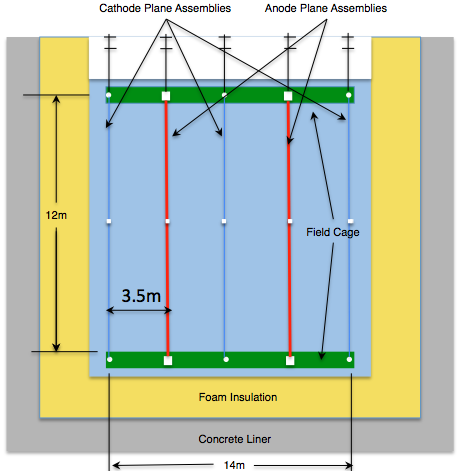
\includegraphics[width=\linewidth]{cpa-apa-arrangement-2014.png}%v5c3-xsect1}
\caption[Cross section of the TPC inside the cryostat]{Cross section of the TPC inside the cryostat.  The length of the TPC is  30~m along the direction of the neutrino beam (into the paper). (Updated 2014) }
\label{fig:tpc-xsect1}
\end{figure}

The TPC's active volume (Figure~\ref{fig:tpc-xsect1}) is 12~m high, 14~m wide and 30~m long in the beam direction. 
Its three rows of CPA planes interleaved with two rows of APA planes 
are oriented vertically, parallel to the beamline with the  
electric field applied perpendicular to the planes.
The maximum electron-drift distance between a cathode and an adjacent 
anode is 3.4~m. Both the cathode and anode plane assemblies are 
2.3~m wide and 6~m high. Two 6-m modules (either APA or CPA)  stack vertically to 
instrument the 12~m active depth. In each row, 13~such stacks are placed 
edge-to-edge 
along the beam direction, forming the 30~m active length of the detector.
Each cryostat houses a total of 52~APAs and 78~CPAs.
Each facing pair of cathode and anode rows are surrounded by a 
``field cage,'' assembled from panels of FR-4 sheets with parallel copper strips connected to resistive divider networks. 

On each APA, four planes of wires cover each side of a frame (the ``wire frame''). See Figure~\ref{fig:tpc-wire-frame-xsect}.
The inner three planes of wires are oriented, going from the inside out: vertically, and at $\sim\pm$36$^\circ$ 
to the vertical, respectively. Each wire is connected to a front-end readout channel.
The wires on the outermost plane are oriented vertically, and are not connected to the readout electronics.
At a nominal wire pitch (center-to-center separation) of 4.8~mm,
the total number of readout channels in an APA is 2560, for a total of 133,120 in each cryostat.
 
\begin{editornote}
  Editor's Note:  The next two paragraphs are now duplicated in the new CE chapter. They should be removed or greatly modified.
\end{editornote}
The readout electronics are optimized for operation in the cryogenic environment.  
The front-end ASIC chip utilizes a mixed-signal design.  
It has 16 channels of preamp, a shaper and an analog-to-digital converter (ADC) in its analog section,  
followed by a large, shared buffer and the digital IO interface. Eight such chips 
are mounted on a single readout board, instrumenting 128 adjacent wires in one plane. 
A digital-processing ASIC with an 8:1 multiplexer on this board further 
increases the multiplexing factor to 128:1, resulting in a single output channel. Data from this output channel will be transmitted 
through two redundant LVDS (low-voltage differential signaling) output cables to two APA-level multiplexing boards.  Each of these boards connects to the 20 front-end readout boards on the APA, and provides a further 20:1 multiplexing.  The output from each of these APA-level multiplexing boards are again duplicated for redundancy.


One cable bundle is planned for each APA to connect to the outside of the cryostat. The bundle will consist of wires for low-voltage power, wire-bias voltages, data out, clock in, digital control IO and an analog monitoring output. Redundant cables will be provided for many of these functions. The 52 cable bundles will be connected through 26 feedthroughs distributed on the roof of the cryostat. Additional feedthroughs will be required for redundant high-voltage connections to the CPAs. 


\begin{editornote}
The wire angle shown in Figure~\ref{fig:tpc-wire-frame-xsect} is 45 degrees whereas as of Jan. 2015 it will be 36 degrees.
\end{editornote}


\begin{figure}[htpb]
\centering
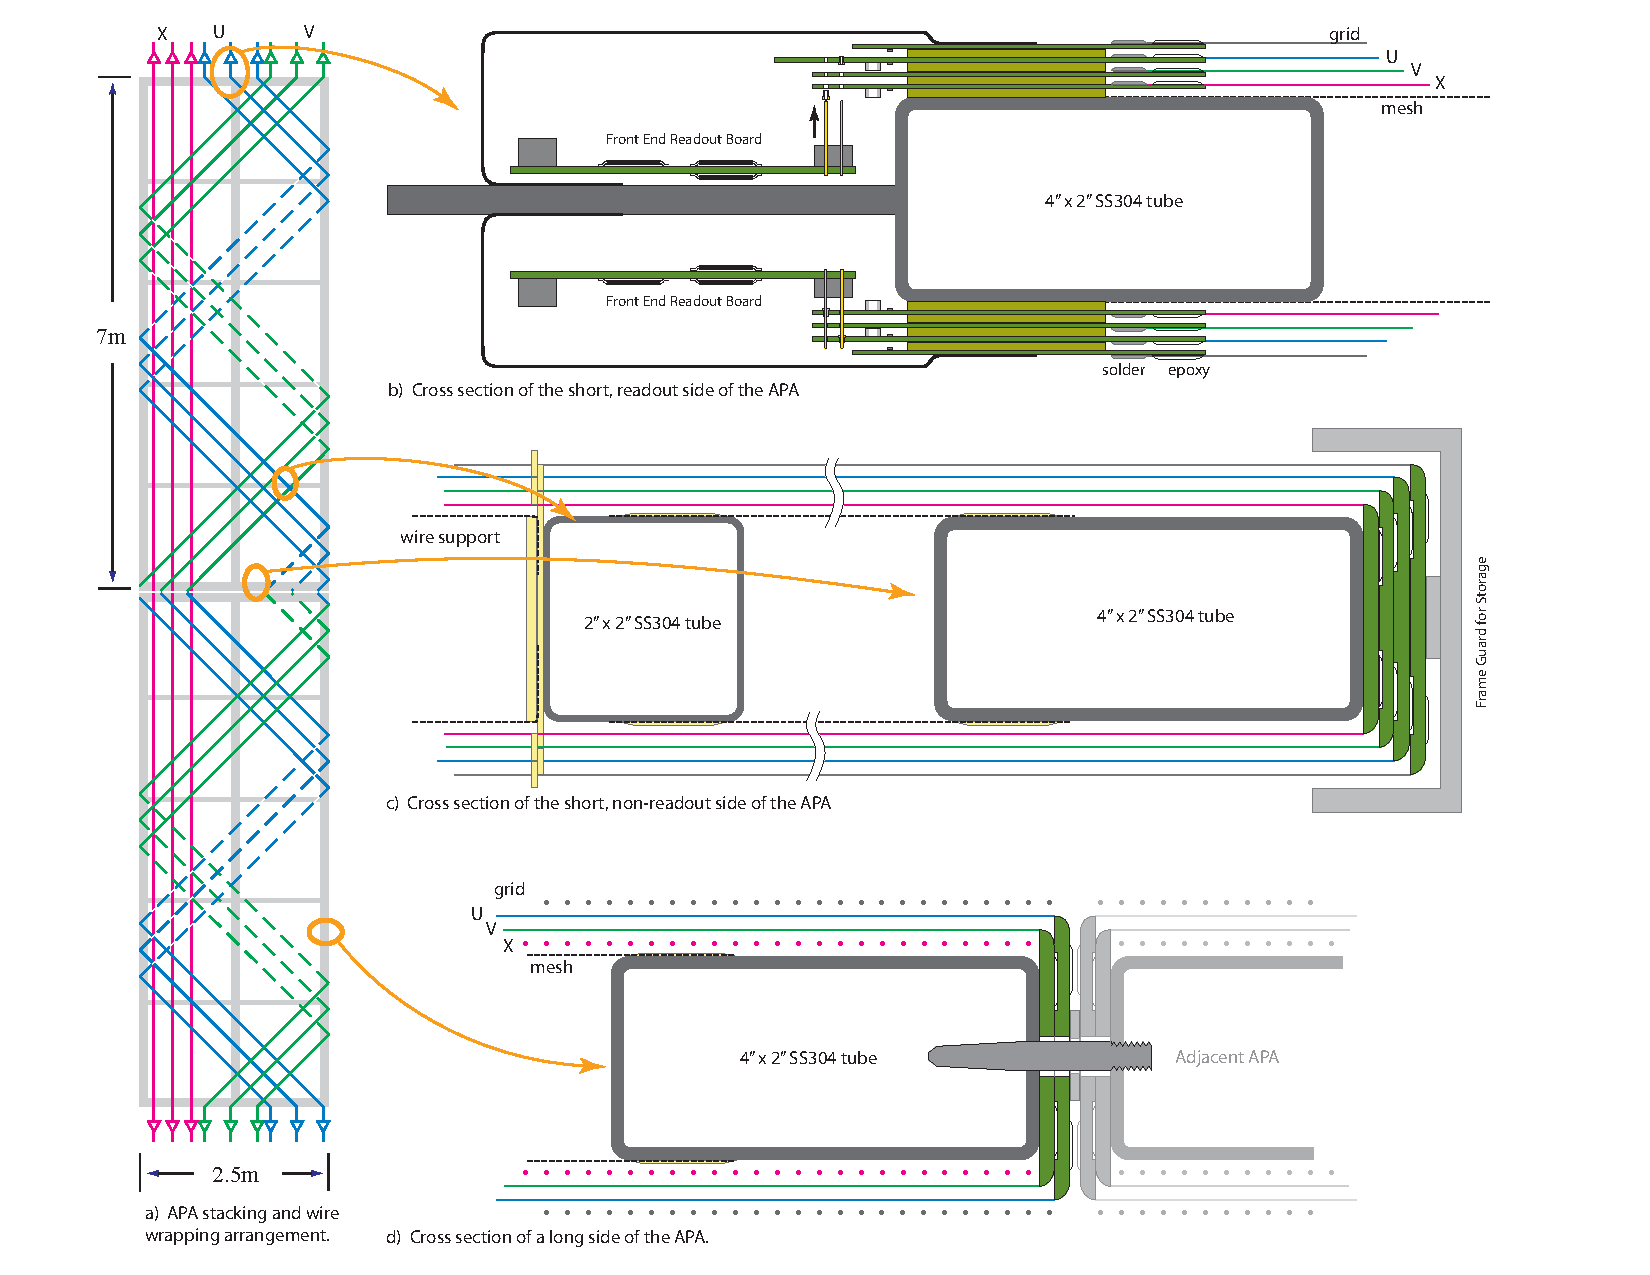
\includegraphics[width=\linewidth]{v5c3-wire-frame-xsects1}
\caption[Illustration of the APA wire wrapping scheme]{Illustration of the APA wire wrapping scheme, and three cross sectional views. (The wire angle shown in this figure is 45 degrees whereas as of Jan. 2015 it will be 36 degrees.)} 
\label{fig:tpc-wire-frame-xsect}
\end{figure}

%%%%%%%%%%%%%%%%%%%%%%%%%%%%%%%%
\section{Design Considerations} 
\label{sec:v5-tpc-reqs-n-specs}

The requirements for the TPC can be found in the requirements documentation \cite{lar-fd-req}. The most significant ones are the following:
\begin{editornote}
  Editor's Note:  Some of these items now appear in the new CE chapter.
  This list below needs to be compared with the corresponding list in CE and revised.
\end{editornote}

\begin{itemize}	
\item Provide the means to detect charged particles in the detector and transmit the detector signals to the Data Acquisition System (DAQ)
\item Meet the physics requirement for electron/photon discrimination;  the TPC wire spacing will be $<$~5~mm
\item Limit variation in the wire sag to $<$ 0.5~mm such that it does not significantly impact the position and energy resolution of the detector
\item Provide redundancy in the discrimination of electrons from photon conversions and ensure long-term reliability over the life of the experiment;  configuration will use three instrumented wire planes
\item Optimize the measurement of high-energy and low-energy tracks from accelerator-neutrino interactions; the wire-plane orientation is optimized for neutrinos in the LBNE energy range
\item Enable the detector to distinguish a Minimum Ionizing Particle (MIP) from noise with a signal-to-noise ratio $>$ 9:1
\item Enable the detector to measure the ionization up to 15 times that of a MIP particle; this is necessary to perform particle identification of stopping kaons from proton decay
\item Enable the in-vessel electronics to operate for the life of the facility
\item Record the wire-signal waveforms continuously without dead time
\item Use only materials that are compatible with high-purity liquid argon

\end{itemize}

%%%%%%%%%%%%%%%%%%%%%%%%%%%%%%%%
\section{Anode Plane Assemblies}
\label{subsec:v5-tpc-chamber-apa}

The APAs are 2.3~m wide, 6~m long, and $\sim 9$~cm thick. The 6-m length is chosen for fabrication purposes and will limit the maximum wire length to 7.3~m (which caps the input capacitance to the preamps to $\sim$165 pF) at a 36$^\circ$ wire angle, and the 2.3-m width is set to fit in a standard HiCube container for storage and transport. 
Each APA is constructed from a framework of light-weight, stainless-steel rectangular tubing, 
with four layers of
wires wrapped over both sides of the frame.  The front-end electronics boards are mounted on 
one end of the wire frame and protected by a metal enclosure.  

%%%%%%%%%%%%%%%%
\subsection{Wires}

The wires used in the TPC must provide:
\begin{itemize}
\item High break load to withstand the applied tension 
\item Good conductivity to minimize noise contribution to the front-end electronics
\item Comparable thermal-expansion coefficient to that of the stainless-steel 
frame to avoid tension change after cool-down
\end{itemize}

Both stainless-steel and copper-beryllium (CuBe) wires are potential candidates.  
Stainless steel was the choice of ICARUS, while a copper-plated 
stainless-steel wire was chosen by MicroBooNE  (to reduce resistance).  Both experiments use a wire-termination 
technique that is labor-intensive and impractical for LAr-FD. Previous experience from FNAL \cite{FNAL-proto-APA} has shown that a CuBe wire under 
tension can be reliably bonded to a copper-clad G10/FR4 (glass epoxy material) surface by a combination of  epoxy (mechanical bonding) 
and solder (electrical connection).  This bonding technique greatly simplifies the electrical 
connection to the readout electronics and it can be easily automated 
with commercial equipment.  Therefore CuBe wire is 
selected as the reference design wire of choice.

At 150~$\mu$m diameter,  the breaking tension of a hardened CuBe wire is $\sim$30~N.  
To ensure no wire breakage in the TPC, e.g. during cryostat cool-down, the nominal operating tension of the wire will be set at 5~N.  Periodic support structures on the wire frame will
limit the unsupported wire length to less than 2~m, resulting in less than 0.2~mm deflection due to gravitational or electrostatic forces.  Wire ends will be glued and soldered (if electrical connection is needed) 
onto printed circuit boards attached to the wire frame.

\begin{figure}[htbp]
\centering
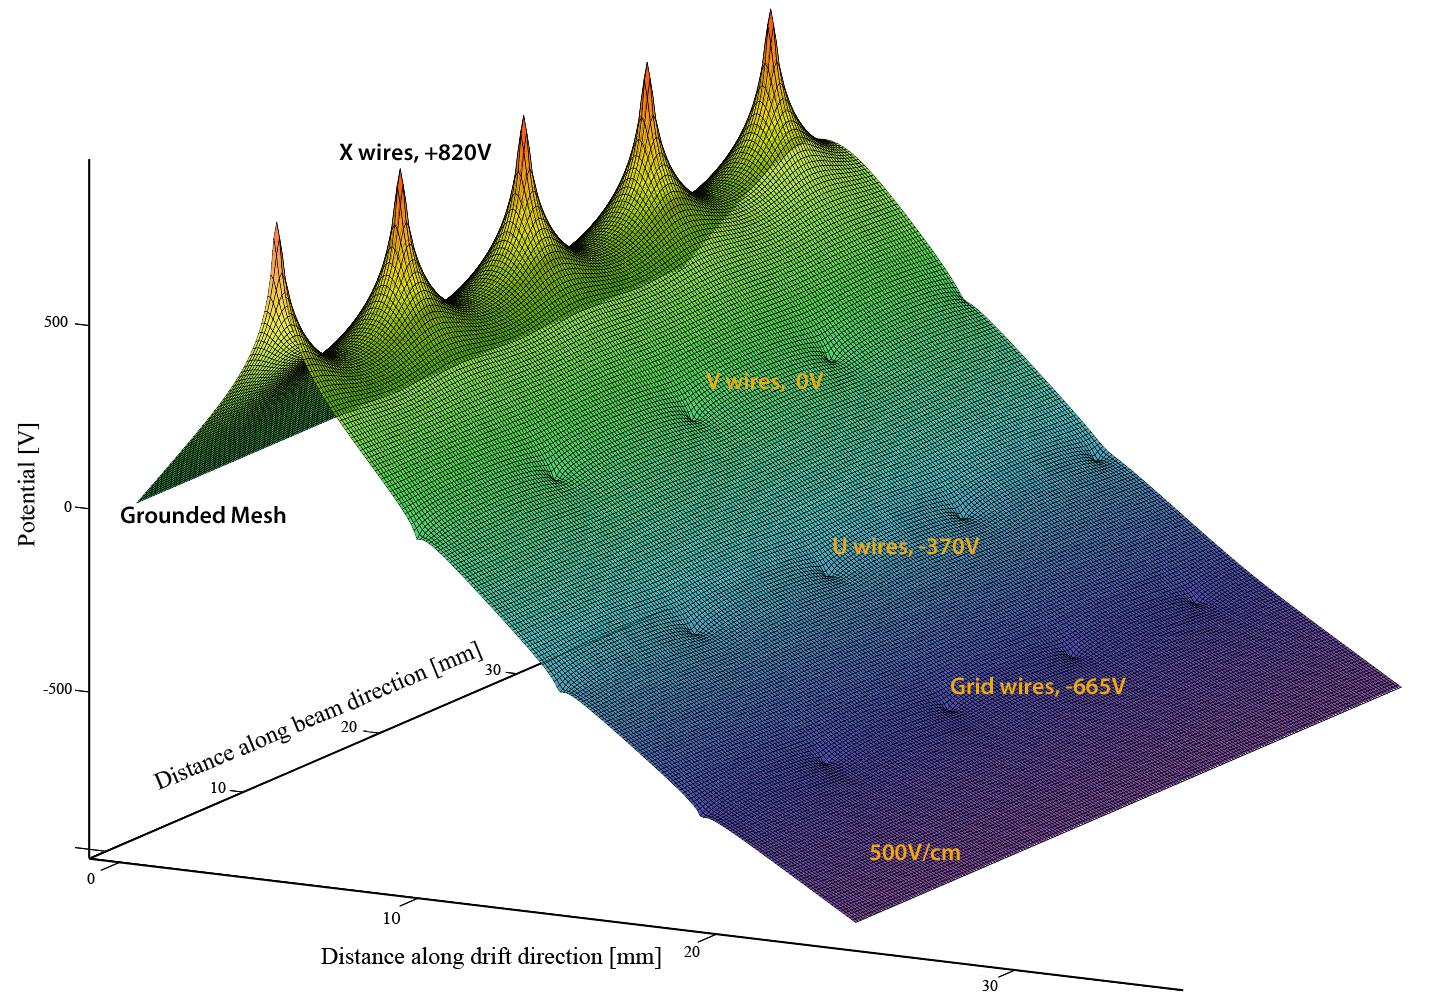
\includegraphics[width=\linewidth]{v5c3-bias-voltages.png}
\caption[Plot of electric potential distribution near the wire planes]{A surface plot of the electric potential distribution near the wire planes.  The voltages on the wire planes are biased to provide complete electron transparency through the first three planes, and complete collection on the fourth plane. }
\label{fig:tpc-bias-voltages}
\end{figure}

%%%%%%%%%%%%%%%%
\subsection{Wire Planes}

\begin{editornote}
Editor's Note: This section needs to be revised based on the 36-degree wire angle.  
\end{editornote}

Four planes of wires are installed on each side of an APA as shown in Figure~\ref{fig:tpc-wire-frame-xsect}.
A nominal wire pitch of 4.5~mm is selected to meet the position resolution  and signal-to-noise ratio requirement. The distance between wire planes is set to 4.8~mm (3/16~in) to use standard printed circuit board thickness, while maintaining optimal signal formation.  These four planes (along the direction of electron drift) are labeled as: the {\em grid plane}, the {\em first induction plane} (U), the {\em second induction plane} (V), and the {\em collection plane} (X).
The wires on the grid and the collection planes
are vertically oriented, while the two induction planes are oriented 
at $\sim\pm$45$^\circ$ to the vertical. This wire layout is shown to be the best for reconstructing beam-neutrino events \cite{wire-orientation}. The wires on the grid plane are not 
connected to the readout electronics; they shield the first induction wire plane from being influenced by distant ionizations. The four wire planes 
will be electrically biased so that electrons from an ionizing-particle
track completely drift past the first three planes and are collected by the 
fourth plane. Calculations show that the minimum bias voltages 
needed to achieve this goal are $V_G= -665$V, $V_U=-370$V, $V_V=0$V and $V_X=820$V 
respectively.  A grounded mesh plane, located 4.8~mm behind the collection plane, prevents the electric field around this set of wires from being distorted by the metal frame structure and the wires on the opposite side of the frame. It also shields the sensing wires from potential EM interferences from the silicon photomultipliers (SiPMs), discussed in Chapter~\ref{ch:photon}, mounted within the frame.  The mesh should be have a wire pitch less than 2~mm to ensure a uniform electric field and a high optical transparency.  Figure~\ref{fig:tpc-bias-voltages} shows the electric potential distribution near the APA frame with the wire planes biased with the appropriate voltages. 

The V wire plane is directly connected to the front-end electronics, i.e. $V_V=0$V, to simplify the coupling and 
reduce the maximum bias voltages on the other planes. The wires on the two induction planes (U \& V) are wrapped in a helical pattern around the long edges of the wire frame 
(Fig.\ref{fig:tpc-wire-frame-xsect}a). This technique makes it possible to place readout 
electronics only at one short edge of a wire frame, enabling joining the APAs on the other three sides with minimal dead space.  It slightly complicates 
the track reconstruction because the U \& V wires are sensitive to tracks on 
both sides of the APA.  The upper APAs in the cryostat will have their readouts
at the top edge of the frame (as shown in Figure~\ref{fig:tpc-wire-frame-xsect}), 
while the lower APAs will mount their electronics at the bottom edge. 

\begin{figure}[htpb]
\centering
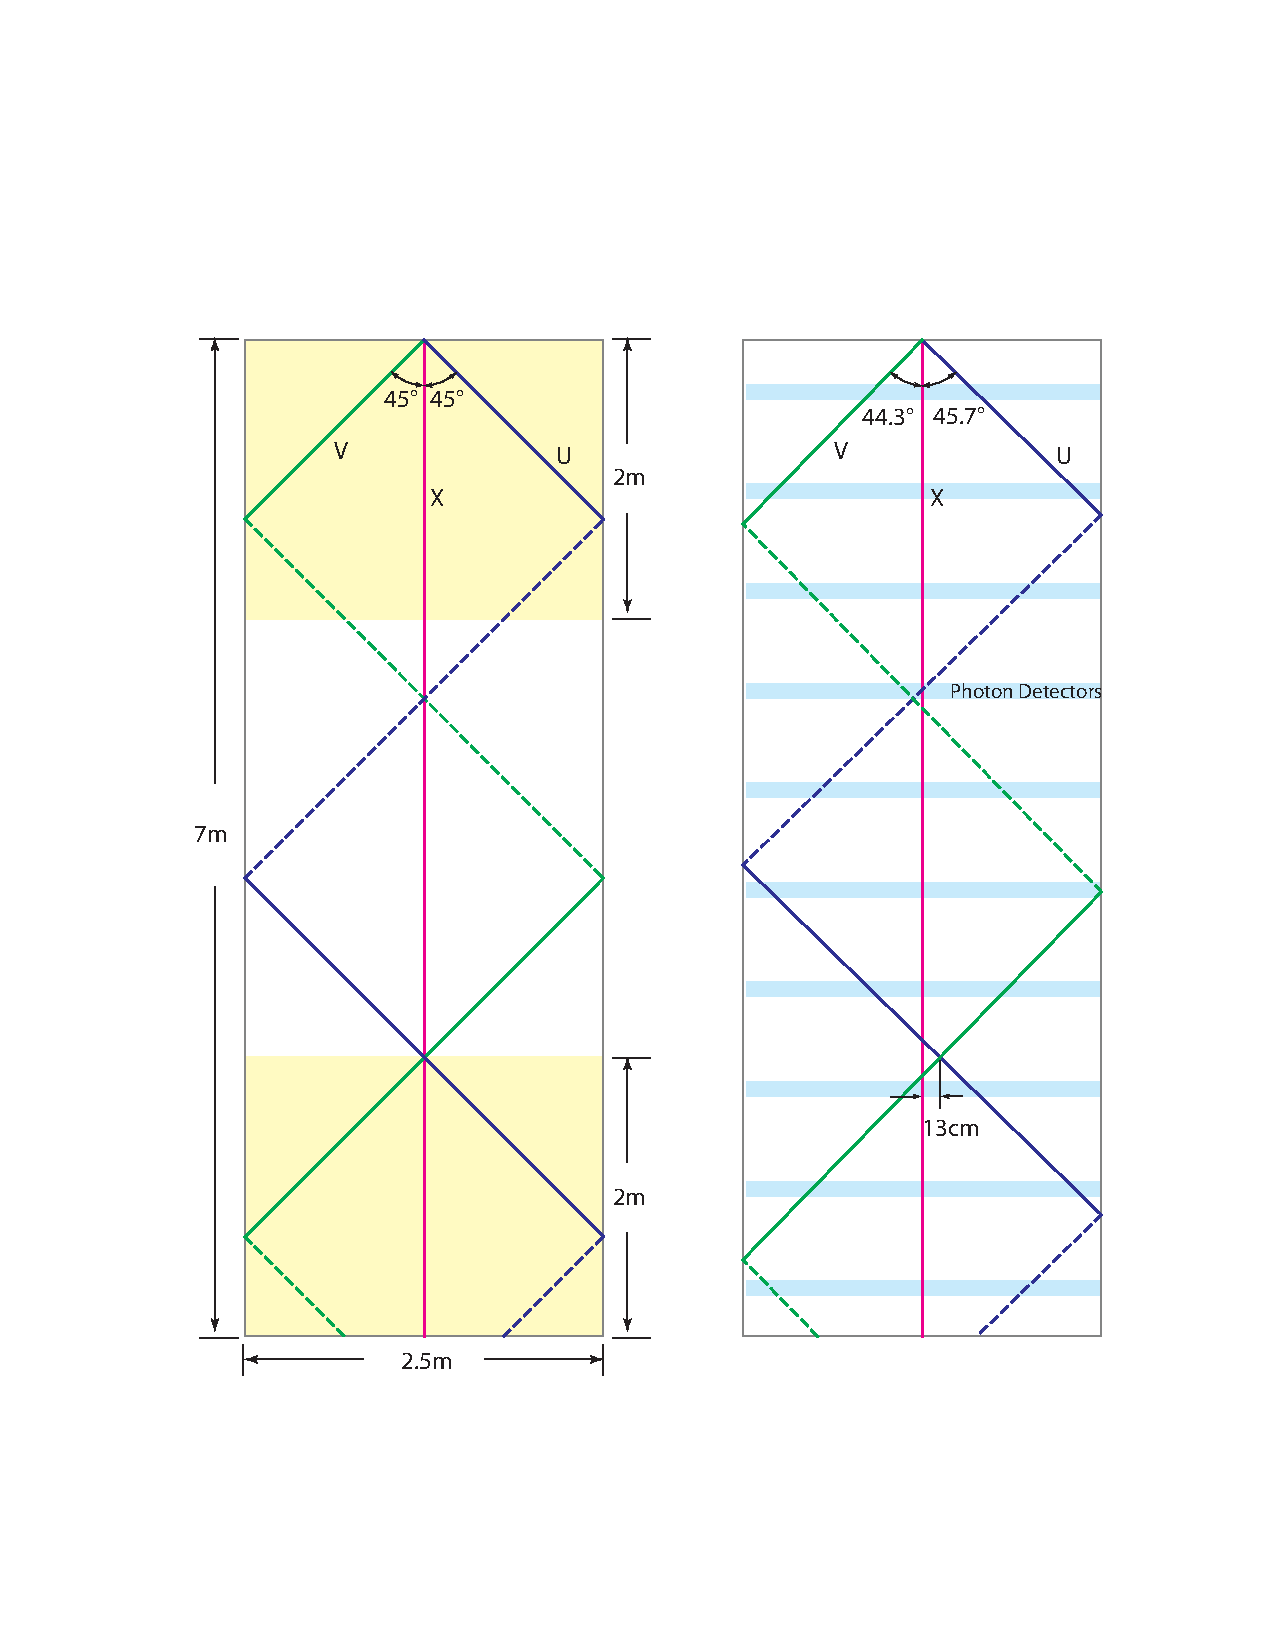
\includegraphics[width=4in]{v5c3-wire-asym.pdf}
\caption[Illustration of ambiguity problem if U \& V wire angles are equal]{Left: illustration of the ambiguity problem if the U \& V wire angles are equal; Right: slightly changing the wire angles and photo detectors help to resolve the problem. }
\label{fig:tpc-wire-asymmetry}
\end{figure}

If the wire angles of the U \& V planes are equal to 45$^\circ$, both wires wrap around the frame one complete cycle, covering a 5-m height, then repeat the same pattern for another 2~m.  An ambiguity problem arises when wire pattern of all three sensing planes in the top 2-m section is identical to that in the bottom 2-m section.  The detector will not be able to tell if a track is in the top or the bottom section of an APA (see Figure~\ref{fig:tpc-wire-asymmetry}).  To resolve this ambiguity, the wire angles of U \& V planes are set slightly differently: $45^\circ\pm\delta$, such that the same three wires do not cross again.   In addition, the multiple photon detectors embedded in the APA frame will help to identify the vertical location of an ionizing track.

The angles and pitches of the U \& V wires are chosen such that (1) a modularity of 128 channels form at the readout end of the APA, with the X wire pitch at 4.5mm; (2) a modularity on the side wrapping boards form with a module length similar to that of the readout board.  The current configuration has the U wires at 45.7$^{\circ}$ from vertical, at a 4.9-mm pitch, while the V wires at 44.3$^{\circ}$ from vertical, and 5.0-mm pitch.


The APA readout electronics are divided into 20 identical modules.  Each module covers 128
readout wires, consisting of 56 X, 36 U and 36 V wires. These 128 readout wires span a width 
of 252~mm.  Using this modularity, the APA's active width is set to 2520~mm. 
There are 1120 X wires, 720 U wires, 720 V wires, and 1120 grid 
wires for each APA.  The total number of readout channels is 2560 per APA. 
The total number of wires per APA is 3680.



\begin{figure}[htpb]
\centering
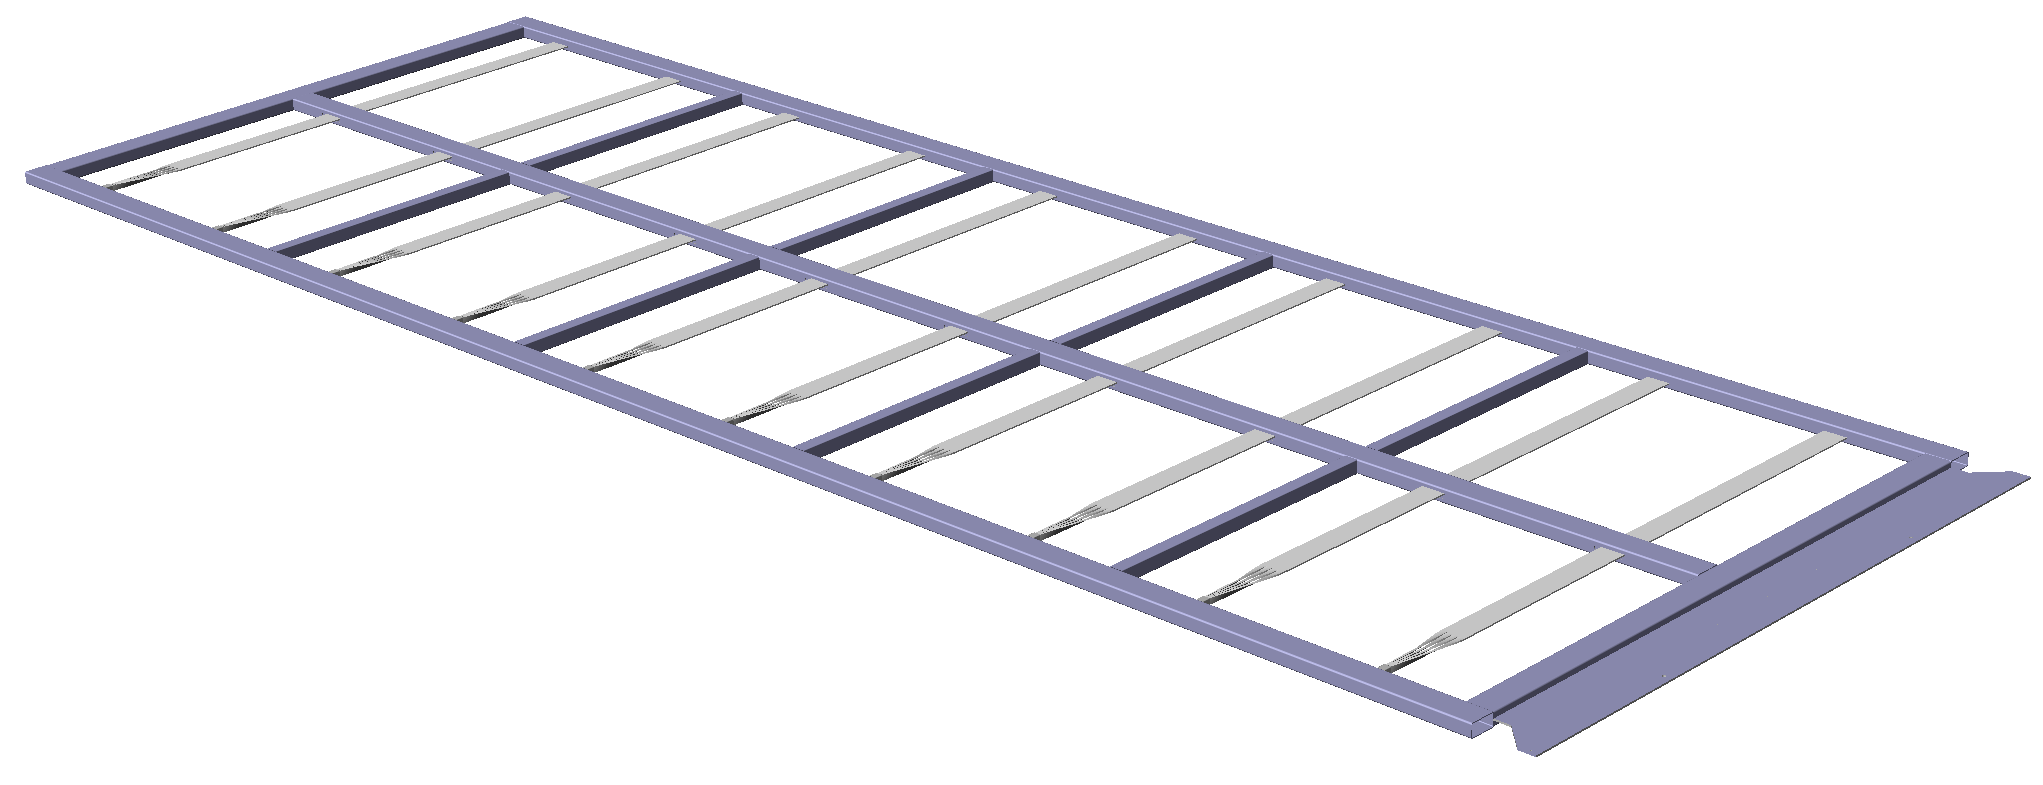
\includegraphics[width=\linewidth]{v5c3-wire-frame}
\caption[Conceptual design of a wire frame]{Conceptual design of a wire frame (shown without wires). The photon detectors are shown installed on the APA frame. }
\label{fig:tpc-wire-frame}
\end{figure}

%%%%%%%%%%%%%%%%
\subsection{APA Frame}

At a nominal wire tension of 5~N, the 3680 wires exert a force of 
$\sim 6.4$~kN/m on the short edges of the APA, and a 
$\sim 2 $~kN/m force on the long edges. The wire 
frame must be able to withstand the wire tension with a minimal 
distortion, while minimizing the thickness of the 
frame to reduce the resulting dead space. A conceptual design 
of the wire frame is shown in Figure~\ref{fig:tpc-wire-frame}.  
It is constructed from all stainless-steel tubes welded in a jig.  Finite element analysis has shown that the maximum distortion of the frame due to wire tension is under 0.5~mm.
The total mass of a frame is $\sim 250$~kg.  All hollow members 
of the frame are vented to prevent the creation of trapped volumes.
The two long outer members of the frame are open-ended, so that signal 
and power cables can be threaded through them to reach the readout 
end of the lower APA.  

%%%%%%%%%%%%%%%%
\subsection{Wire Wrapping Around an APA}


\begin{figure}[htpb]
\centering
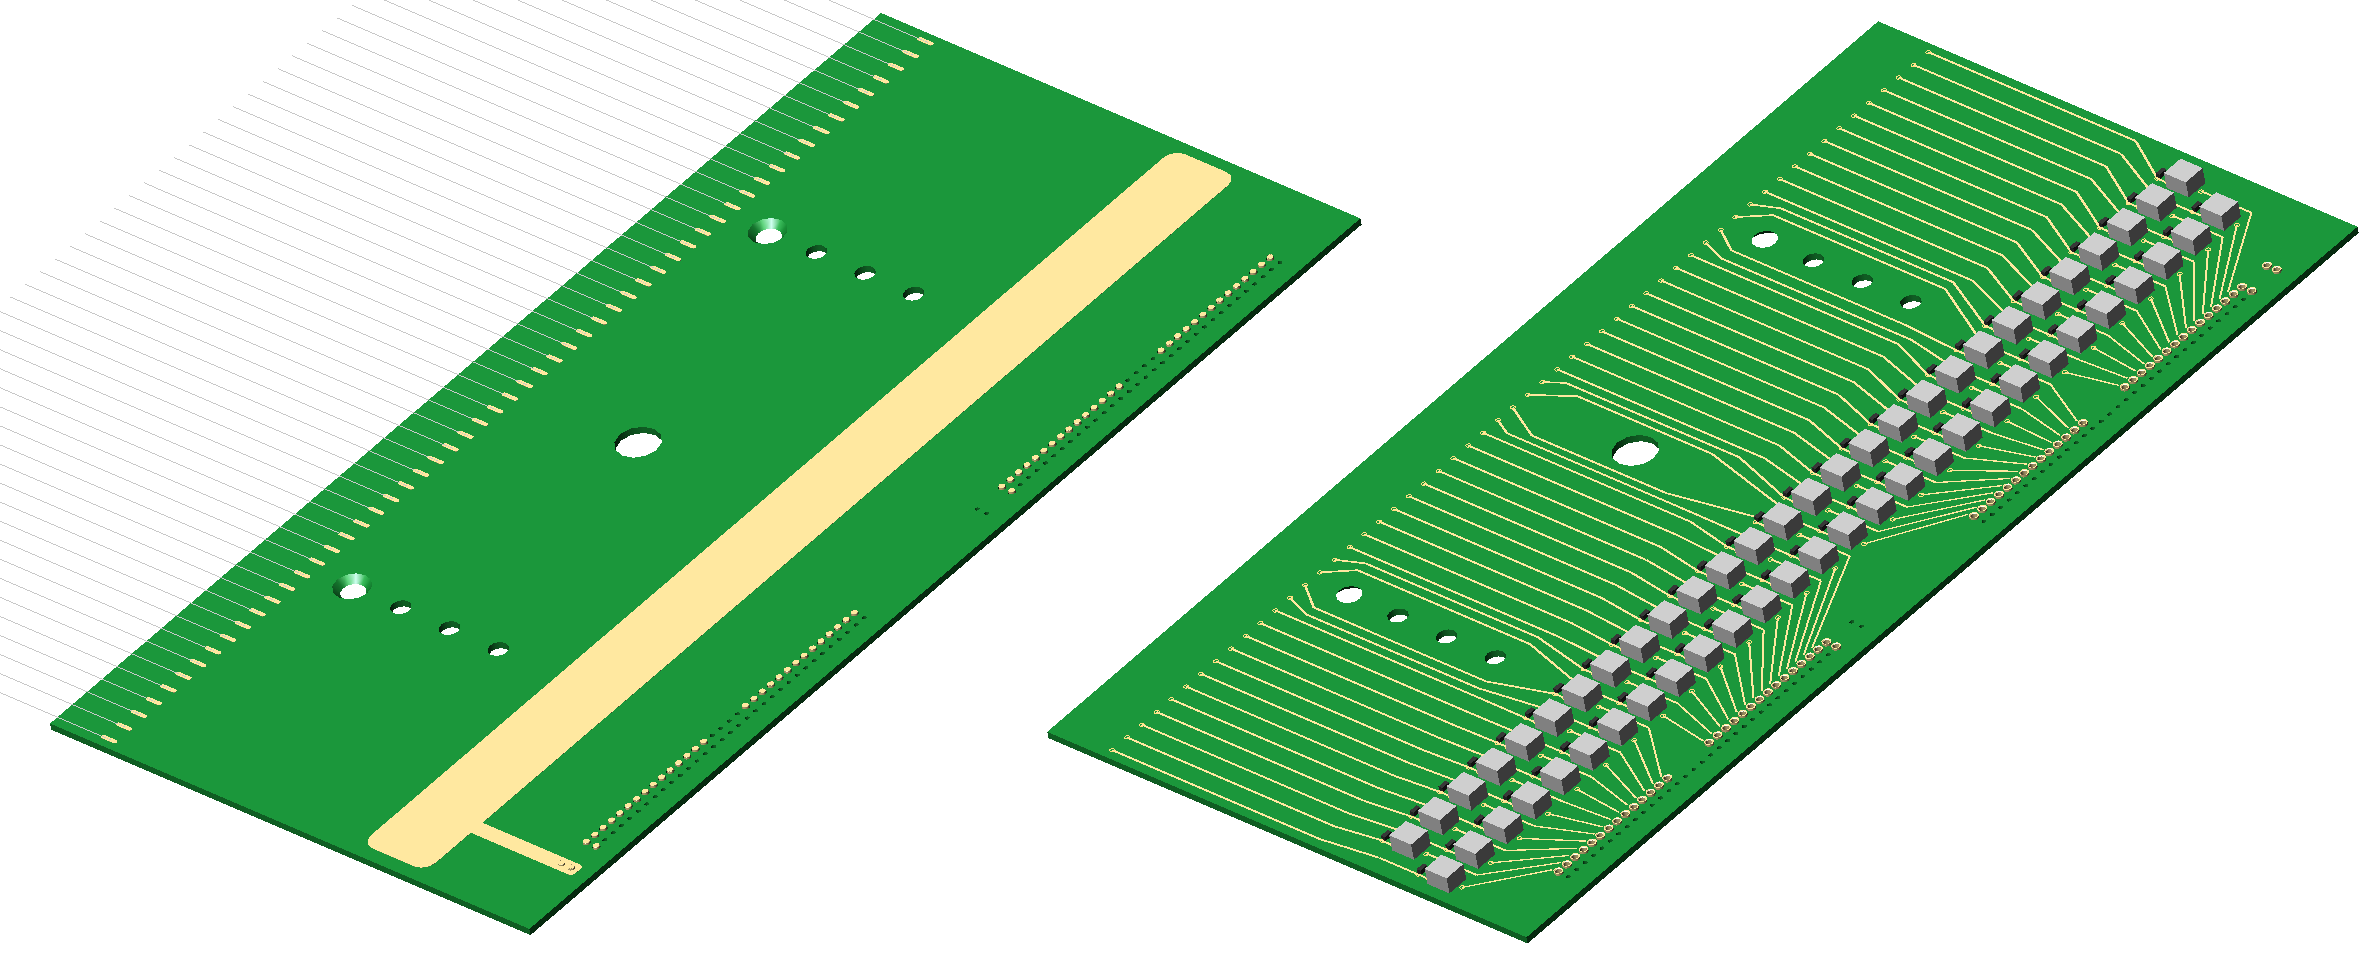
\includegraphics[width=\linewidth]{v5c3-x-top-board}
\caption[Conceptual design of a wire bonding board for the x wires]{Conceptual design of a wire bonding board for the x wires. Left: An array of wires are glued on the leading edge of the top surface, and then soldered onto the soldering pads; Right: the bottom side of the board has the RC network for the bias voltage. }
\label{fig:tpc-wire-board-x}
\end{figure}


Figure~\ref{fig:tpc-wire-frame-xsect}b-d shows three major cross sections of an APA.  The top figure is the cross section of the readout end of an 
APA.  The four planes of wires are attached to their respective 
wire-bonding boards through a combination of epoxy and solder.
Figure~\ref{fig:tpc-wire-board-x} shows both sides of the board for the x wires.  
The wires are wound on the top surface of the board (left) using a winding machine.  The wires are then glued down with a bead of epoxy at the leading edge of the board.  After the epoxy has cured, the wires are soldered onto the copper pads under each wire, and the wires are cut beyond the pads.  On the bottom of this board, the copper traces connect the wires to the bias voltage supply through an RC network.  The resistors in this network have values about 20 M$\Omega$, such that in the event that a wire from a different plane breaks and is shorted to these wires, the bias voltages on the rest of the wires will not be affected. The AC-coupled signals from the wires are connected to sockets that will mate with the front-end readout boards.

Similar boards for the U \& V planes are aligned and stacked above the X boards.   An array of pins on the front-end readout boards is pushed through the stack of wire bonding boards, making electrical connection between the readout electronics and the matching wires. These readout boards, as described 
in Chapter~\ref{ch:ce}, process the analog signals from the wires and transmit 
the digital information through feedthroughs to the DAQ system outside 
the cryostat.  The electronics on the readout boards dissipate an estimated $\sim$60~W of heat per APA and may generate a small quantity of argon bubbles.
Two stainless-steel covers are placed over the readout boards to contain 
the bubbles and direct them to the gas volume of the cryostat. In the case of the lower APAs, the bubbles, if not already recondensed, will be funneled through the vertical hollow frame members to the top of the cryostat.

Figure~\ref{fig:tpc-wire-frame-xsect}c shows the cross section of the short, non-readout end 
of an APA. All wires are mechanically terminated on this end on the four layers 
of wire-wrapping boards.  No electrical connections are needed. 


Figure~\ref{fig:tpc-wire-frame-xsect}d shows the cross section of a long edge of an APA. 
Only two layers (U \& V) of wire wrapping boards are needed here. The wire-wrapping boards are 
made from printed circuit boards, shown in Figure~\ref{fig:tpc-wire-board-u-side}. The boards are attached to the APA frame, and then a winding machine wraps a wire around the APA in a helical fashion, placing the wire into the grooves on the edges of each board. After winding, the wires are glued down to the wire-wrapping boards near the grooved edges.  To clear the mounting holes on the board, a few wires are soldered onto the copper pads, and cut, leaving the copper traces to bridge the connection.  
 
Figure~\ref{fig:tpc-APA-corner} is a closeup view of a corner of an APA frame with some wires and various wire bonding boards to demonstrate the assembly.
   
After the grid plane wires are placed on the APA,  metal guards are placed along the three wrapped edges of an APA.  These guards protect the fragile wires during APA handling, storage and transport.


\begin{figure}[htpb]
\centering
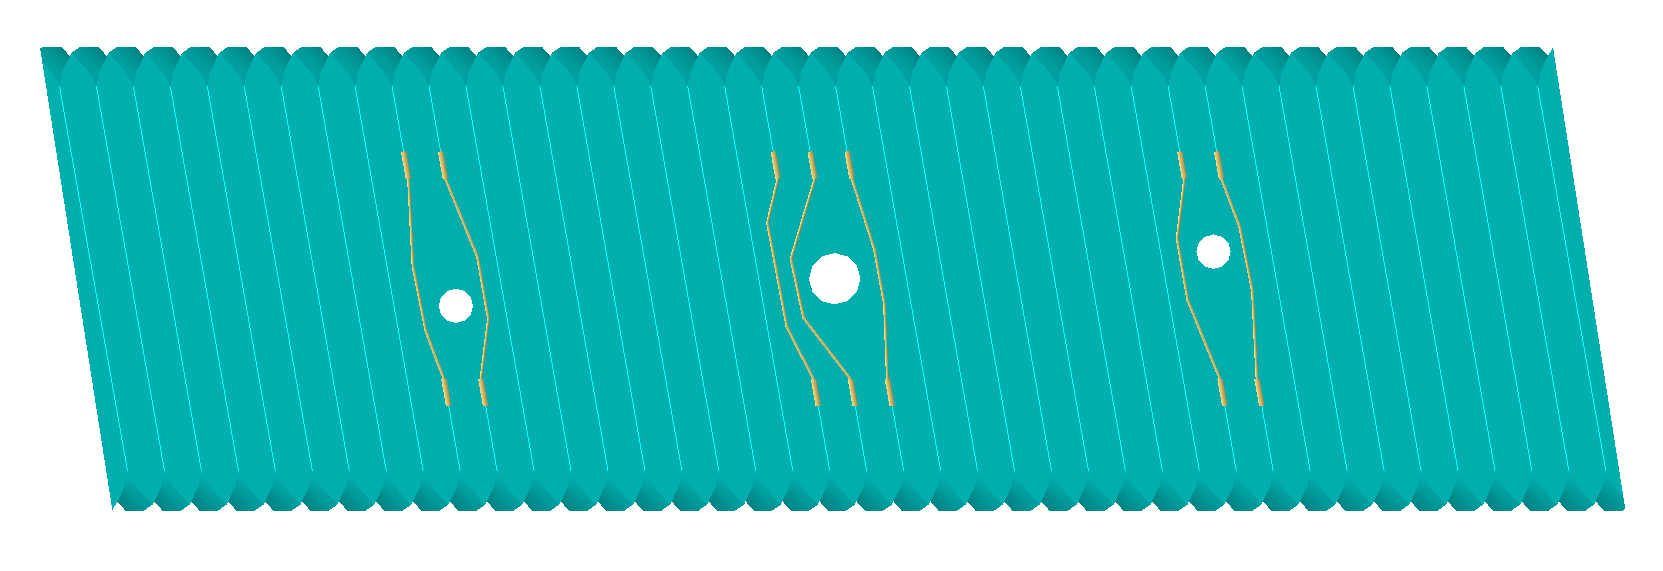
\includegraphics[width=\linewidth]{v5c3-u-side-board}
\caption[Concept of wire wrapping board for U wires on long edge of APA]{Conceptual design of a wire wrapping board for the U wires on a long edge of an APA.  The light cyan colored lines represent the wires wrapped over the board surface.  Some wires near the mounting holes must be soldered to the copper traces and then cut.}
\label{fig:tpc-wire-board-u-side}
\end{figure}

\begin{figure}[htbp]
\centering
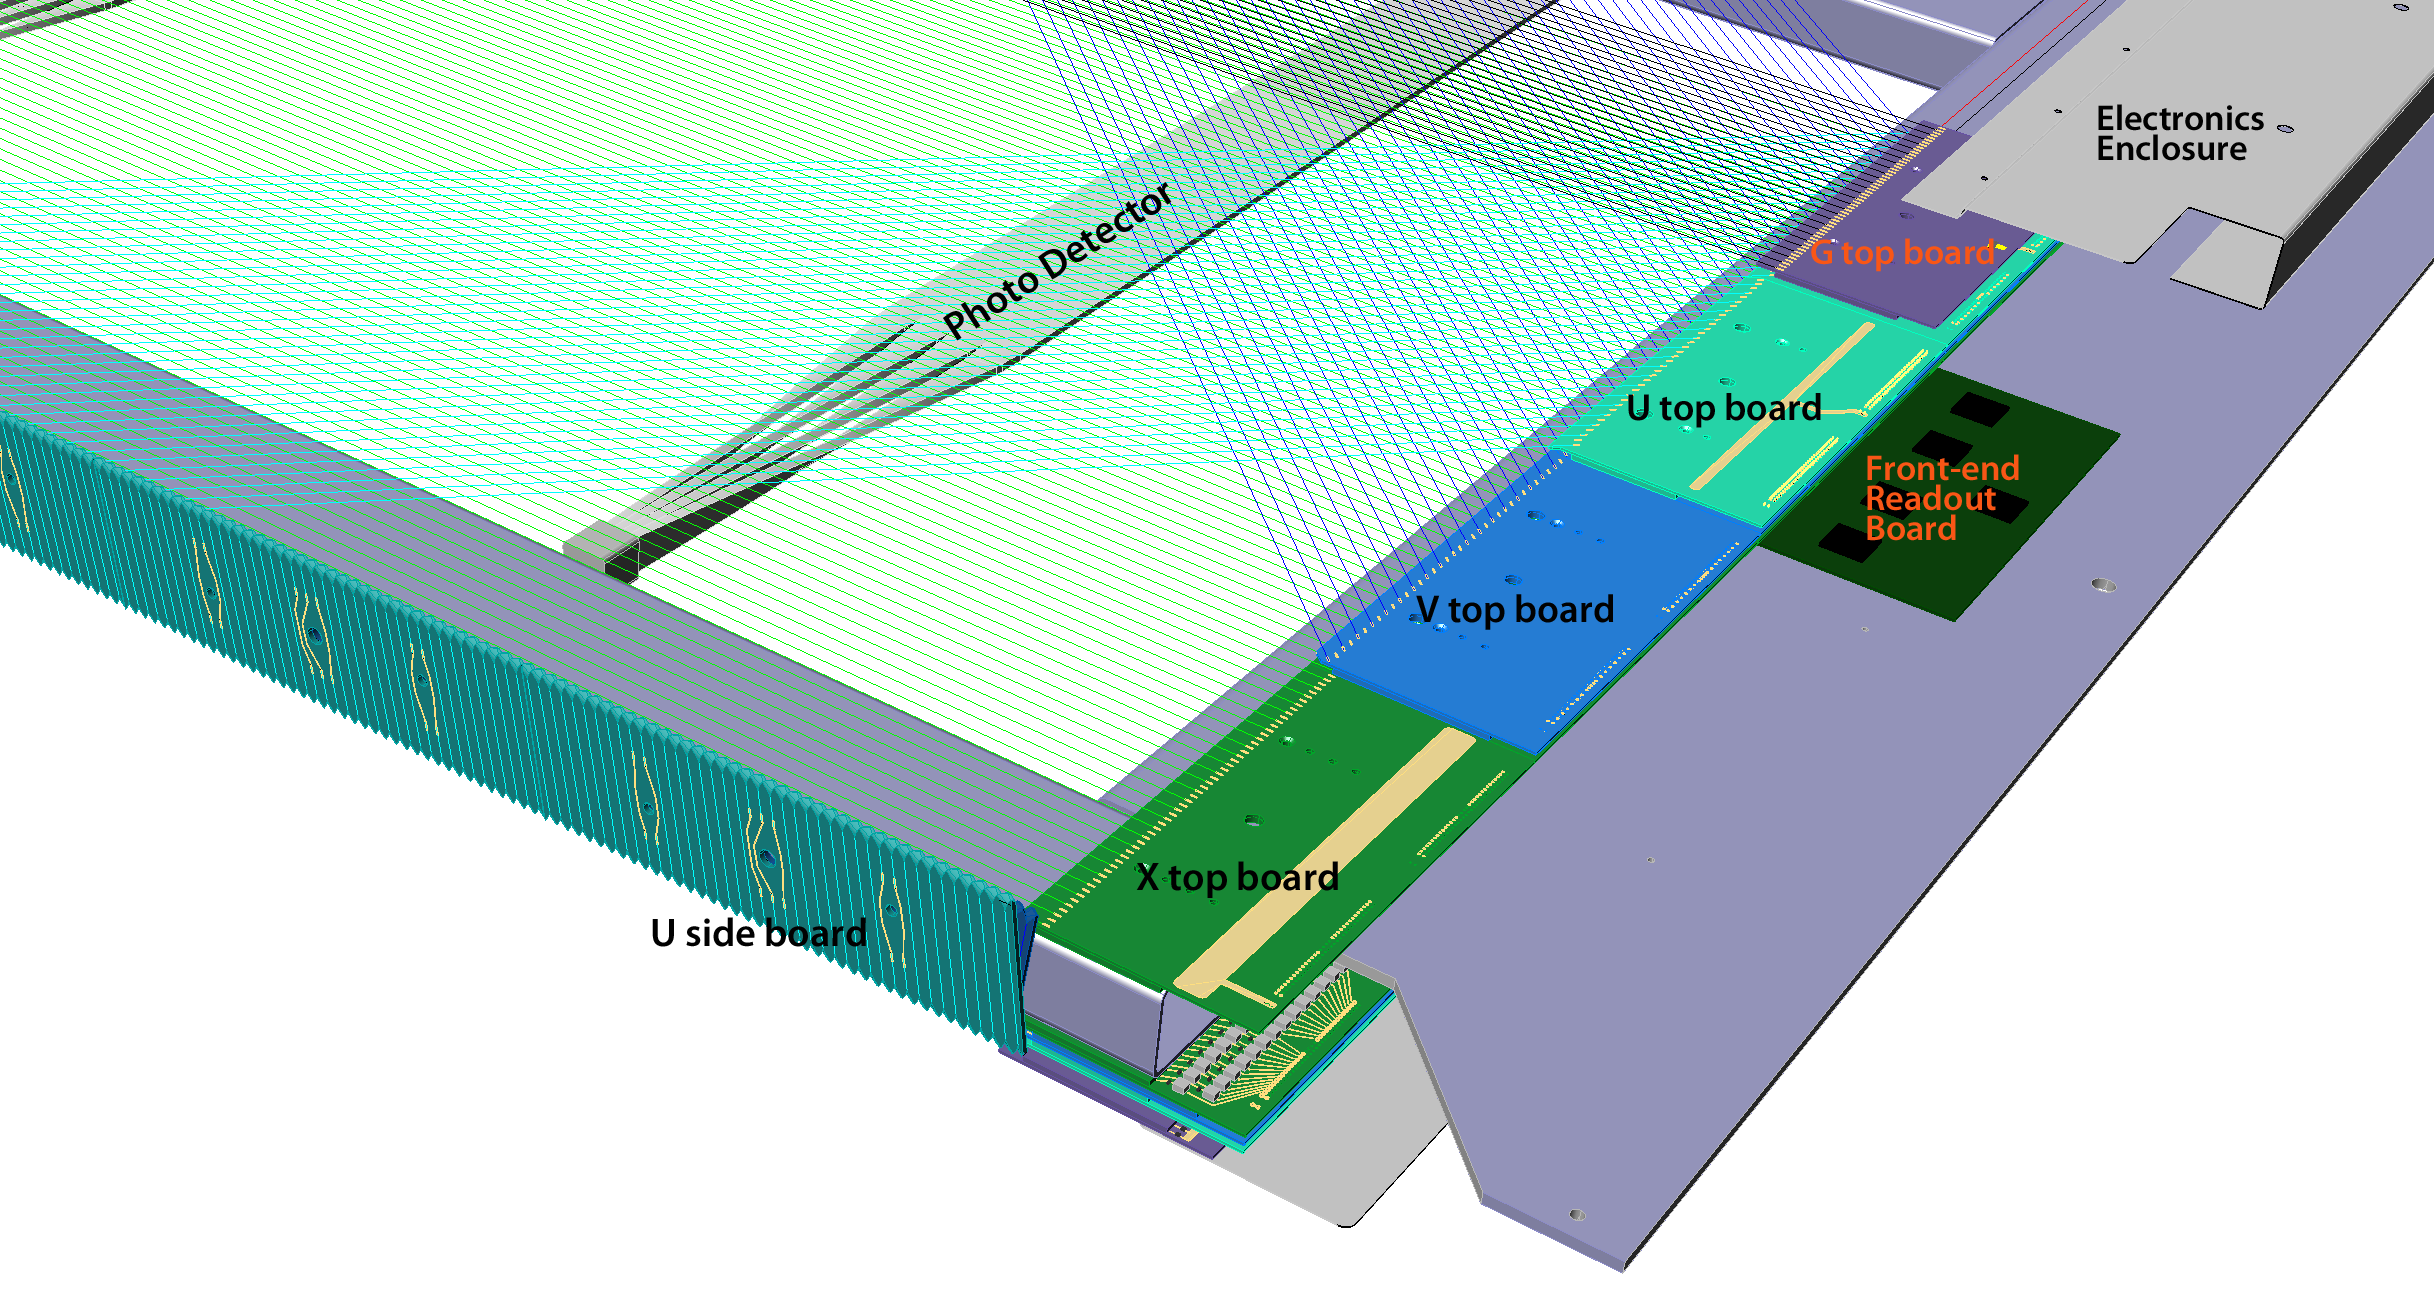
\includegraphics[width=\linewidth]{v5c3-APA-corner-view.png}
\caption[Closeup view of a partially assembled corner of an APA]{A closeup view of a partially assembled corner of an APA.  For clarity, only every other wire is shown in this illustration.  }
\label{fig:tpc-APA-corner}
\end{figure}

%%%%%%%%%%%%%%%%
\subsection{Wire Supports on Inner Frame Members}

The left of Figure~\ref{fig:tpc-wire-frame-xsect}b also shows the wire-support 
structure mounted on one of the inner horizontal frame members. 
A detailed rendering of this concept is illustrated in 
Figure~\ref{fig:tpc-wire-support}. The support structure is composed of
strips of thin fiberglass boards, with notches machined at specific 
intervals. The support strips for X plane is directly mounted on the 
inner frame members.  After all X wires have been placed into the slits, 
the V support strip (shown in green) is glued onto the tips of the 
X strips, trapping the X wires in position.  After the V wire are placed 
into the slits, the U support strip (identical to the V strip) is glued 
to the V strip, trapping the V wires. These structures are 
repeated four times along the 7-m length of an APA, limiting the unsupported 
wire length on any wire plane to $< 2$~m, while introducing 
only millimeter-scale dead regions. These wire supports play a key role 
in minimizing wire deflection due to gravity and electrostatic force, 
enabling the use of a moderate wire tension and reducing the 
risk of wire breakage. 


\begin{figure}[htpb]
\centering
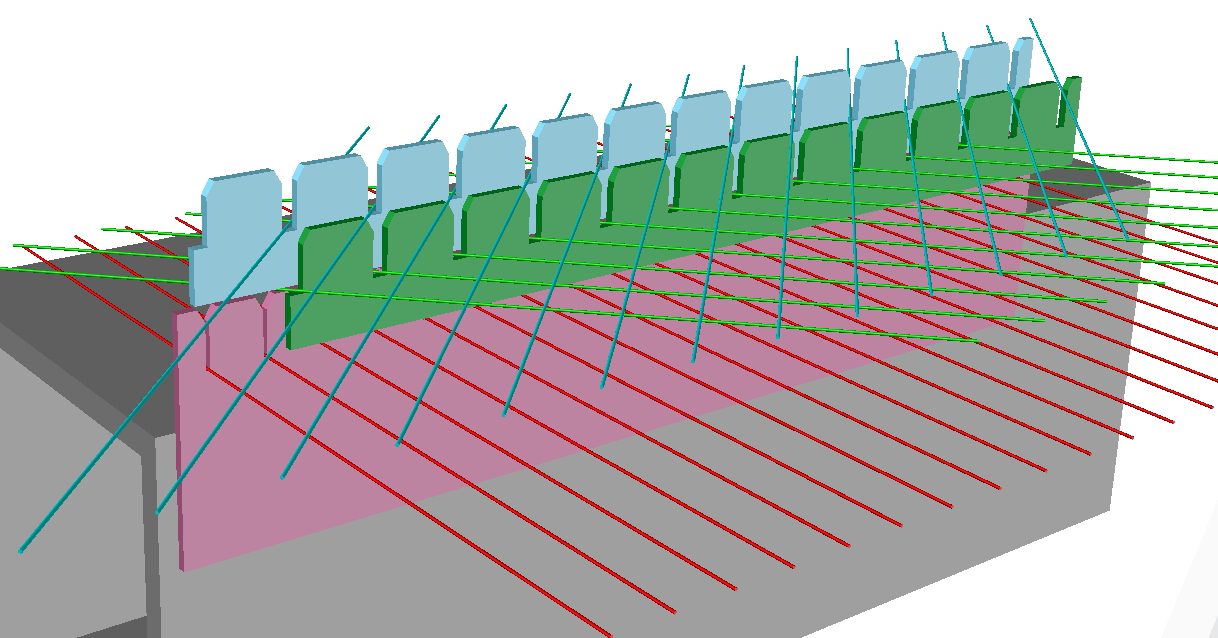
\includegraphics[width=\linewidth]{v5c3-wire-support}
\caption[Conceptual design of the wire support for the U, V \& X wires]{Conceptual design of the wire support for the U, V \& X wires.  
Similar structures will be used to support the grid wire plane.}
\label{fig:tpc-wire-support}
\end{figure}

\begin{figure}[htpb]
\centering
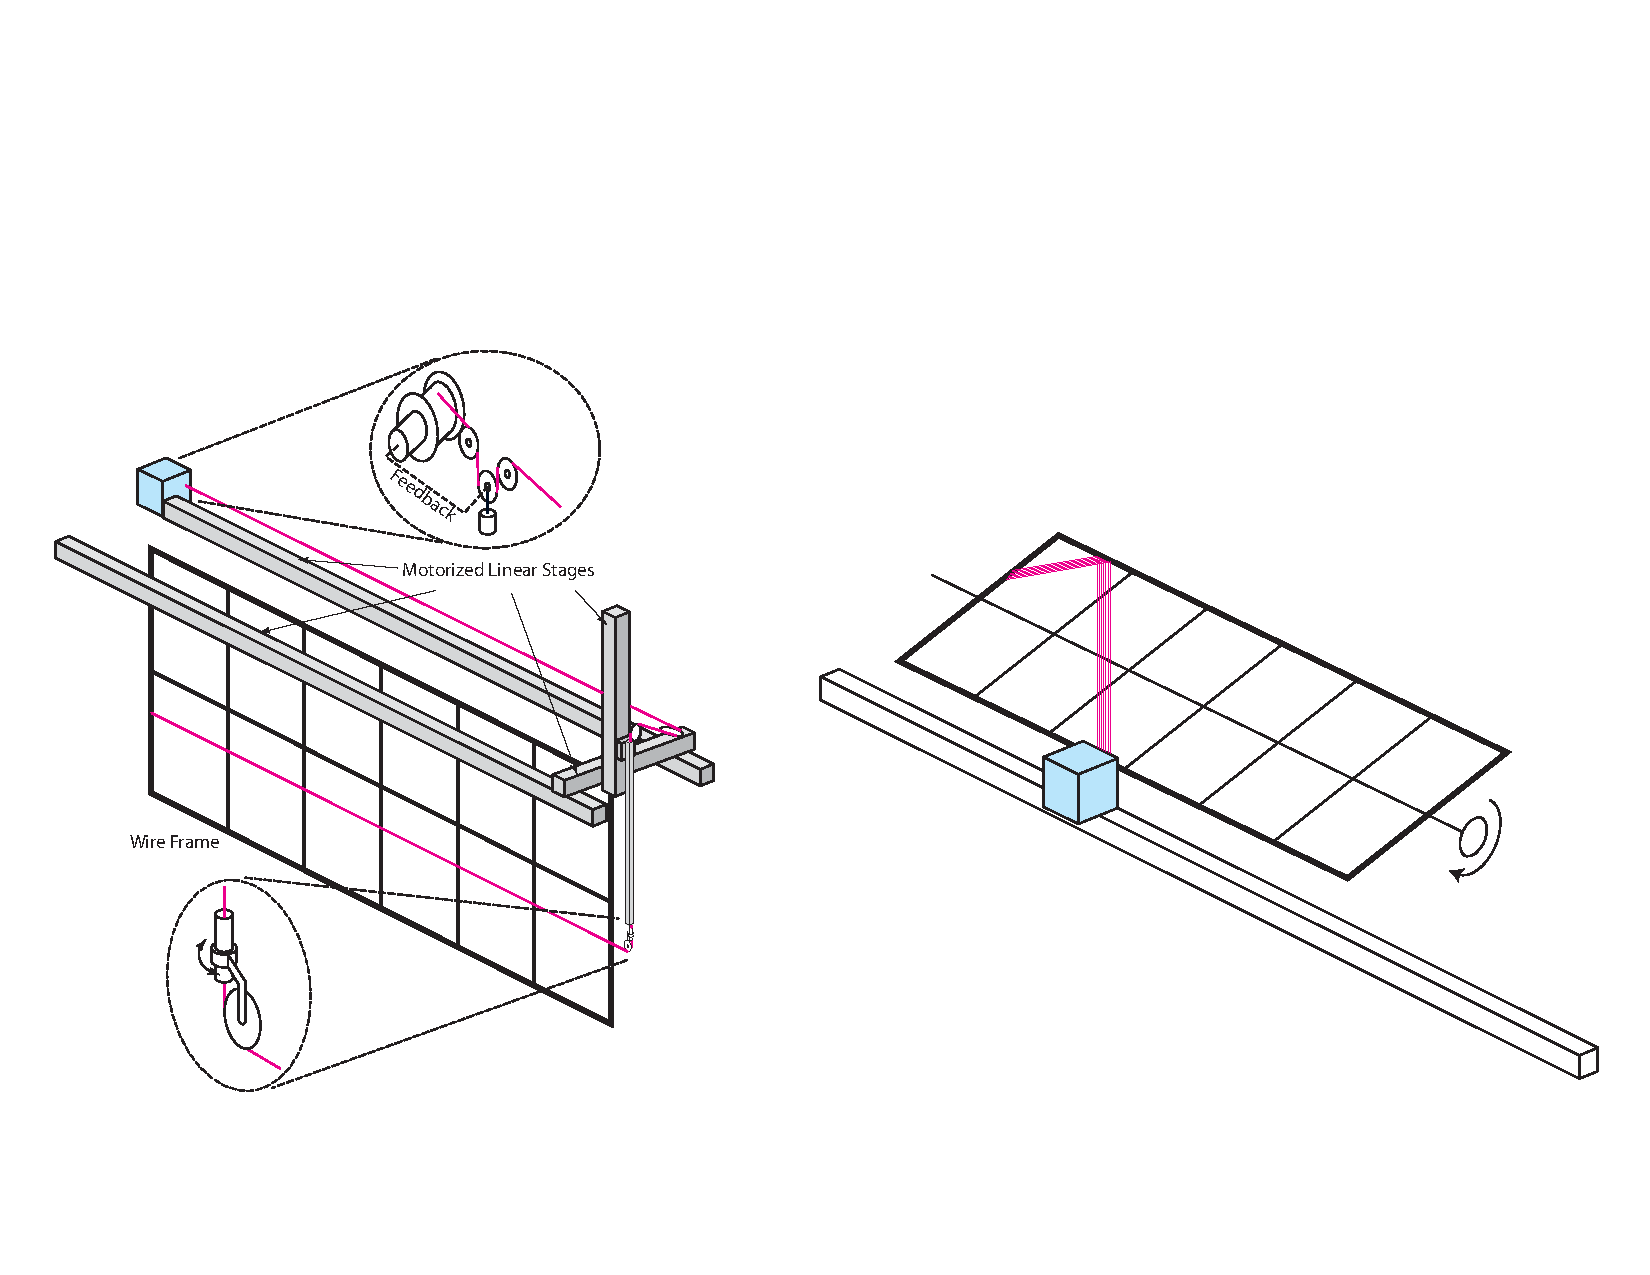
\includegraphics[width=\linewidth]{v5c3-tpc-winding-machines}
\caption[Two winding machine concepts]{Two winding machine concepts. The left figure is for the X and grid wires.
The right figure is for the U \& V wires.  The 'blue boxes' are wire spools 
with automatic tension control.}
\label{fig:tpc-winding-machine}
\end{figure}

%%%%%%%%%%%%%%%%
\subsection{Wire-Winding Machines}

Two winding machines will be constructed to lay the 3680 wires on each APA. 
Their working concepts are illustrated in Figure~\ref{fig:tpc-winding-machine}. 
For the X and the grid wire planes, (left figure), the wire frame will be standing on 
one of its long edges, while a wire is wrapped around the frame using a commercial
3-axis gantry robot. A wire-tension controller maintains the wire 
tension and feed rate of the wire off the spool. Although the entire plane of 
wires can be wound in one pass, a more fault-tolerant procedure is to 
pause the winding machine periodically and solder the last wire onto the frame.
This intermediate soldering step will prevent the unraveling of a large section 
due to an accidental broken wire.  
The winding machine for the U \& V planes will wrap a group of wires ($\sim 10$) as a band in each pass.
An automatic soldering robot will solder the wire ends after the group of wires has been laid down on one side of the frame. 
A wire-tension measuring device will scan the newly placed wires and record 
the wire tension of each wire. Any wires with abnormal tension will be 
replaced manually.  

%%%%%%%%%%%%%%%%
\subsection{Alternative APA Construction}

\begin{editornote}
  Editor's Note:  The APA size described in this section does not reflect the change from 2.5 m $\times$ 7~m  to 2.3 m $\times$ 6 m.
\end{editornote}

The APA design described above requires two customized machines capable of placing wires directly on the 2.5~m $\times$ 7~m APA frame with a precision of the order of 1~mm.  Cleaning the solder flux off the APA after wire bonding also poses a challenge on an object this size. An alternate APA design is under development to alleviate these difficulties.  In this design, the APA frame dimensions and the wire geometry remain  approximately the same, but the wires are attached to the APA frame in a two-step process.

The first step is to bond a group of wires ($\sim$64) with epoxy and solder on two FR-4 boards to form a wire module.   The second step is to mount all the assembled wire modules onto an APA frame using a stretching table.  The wire lengths in each wire module are determined in such a way that when a module is mounted on the frame, all wires will reach a uniform tension of 5~N.  Jumper cables interconnect the corresponding U or V wire modules along the two long edges of an APA to complete the helical wire wrapping pattern electrically.
The assembly of an APA frame  using prefabricated modules will be easier and faster than direct winding on the big frame.  If a wire is broken while being attached to the frame, it is relatively straightforward to replace the affected wire module. The details of APA assembly are shown in Figure~\ref{fig:tpc-APA-AD1}.  
 
\begin{figure}[htpb]
\centering
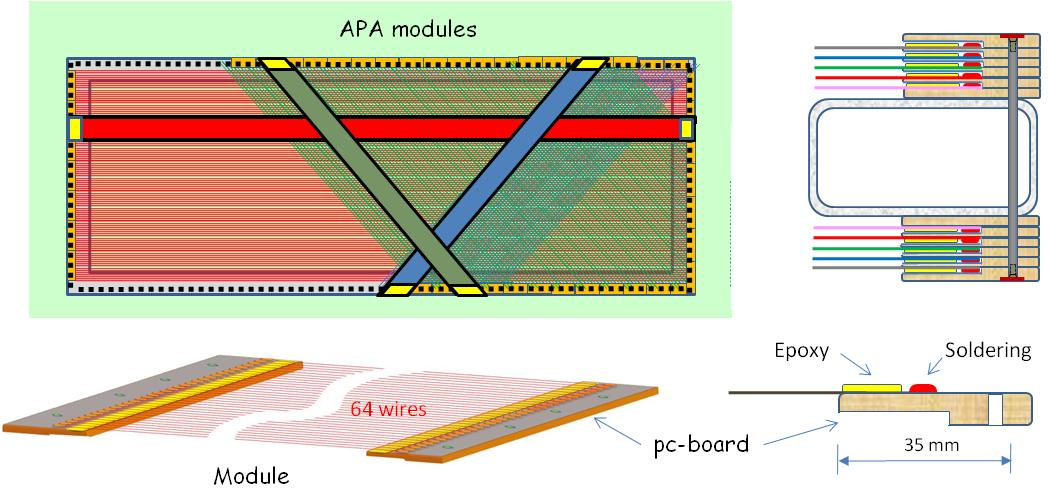
\includegraphics[width=\linewidth]{v5c3_APA_AD1}
\caption[Concept of the alternative APA wiring scheme]{Concept of the alternative APA wiring scheme using pre-assembled wire modules}
\label{fig:tpc-APA-AD1}
\end{figure}

One major drawback of this alternative design is a relatively large dead space between any APA joints ($\sim 2 \times 35$~mm) due to the FR-4 board size.  The electric field in the drift region directly above the FR4 boards will have some irregularities, causing minor distortion to the track trajectories. To eliminate these problems, additional special wire modules could be placed over the dead region at the APA edges. For example, a module with two layers of 18 wires ($\sim$90~mm wide) would completely cover the FR-4 boards between two APA frames. The upper layer wires maintain the uniform drift field, collect the electrons, and provide the X position information, just like the regular X readout wires. The obtained X coordinates and charge information partially restore the detector sensitivity at the APA joints. The scheme with additional wire modules is shown in Figure~\ref{fig:tpc-APA-AD2}. 
                   
\begin{figure}[htpb]
\centering
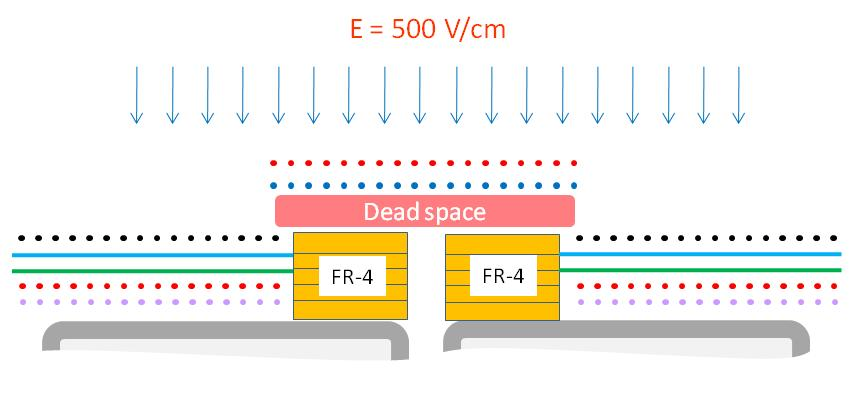
\includegraphics[width=\linewidth]{v5c3_APA_AD2}
\caption[Illustration of dead space above FR-4 boards and possible solution]{Illustration of dead space above FR-4 boards and possible solution with installation of two additional wire planes above.}
\label{fig:tpc-APA-AD2}
\end{figure}


Using the wire geometry shown in Figure~\ref{fig:tpc-APA-AD2} the bias voltages for wire planes have been defined and electric field strength calculated in 2D. The calculation confirmed that the drift field above the FR-4 boards is uniform, and full collection of electrons can be achieved on the additional wire modules. From past experience,  the electric field is not expected to change very much in a 3D simulation. Nevertheless, it is necessary to develop a full 3D model for more accurate field calculations and simulation of electron drift in real APA geometry.
  
One of the advantages of this alternative design is the modularity of wire planes that will simplify the wire placement and APA assembly. The winding procedure becomes simple and reliable and a simple winding machine with replaceable wheels is required. The module production could be done at several sites to accelerate the APA assembly schedule. The completed modules will be cleaned in an ultrasonic bath, dried in a vacuum oven and stored in dry air. A set of tests will be performed to ensure that modules meet the technical specifications. The winding scheme for module fabrication is presented in Figure~\ref{fig:tpc-APA-AD4}.
                              

\begin{figure}[htpb]
\centering
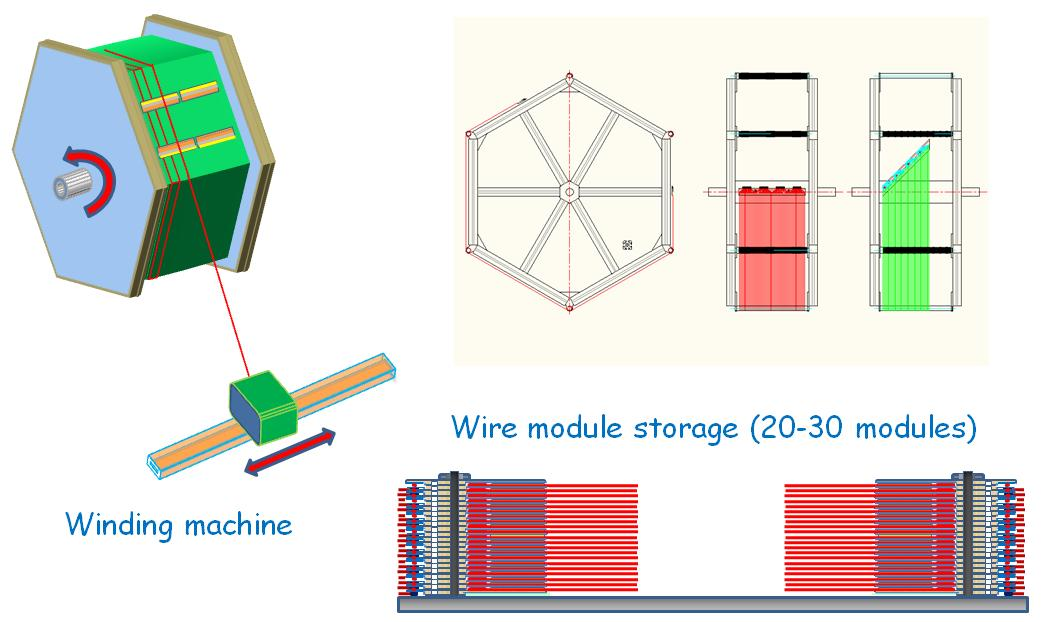
\includegraphics[width=\linewidth]{v5c3_APA_AD4}
\caption[Conceptual designs of the wire winding machine and wire module storage fixture]{Conceptual designs of the wire winding machine and wire module storage fixture.  Upper left: the fabrication of the wire modules are accomplished by attaching the wire module boards on to a large drum with specific circumference, and laying the wires over the boards at a constant pitch.  Upper right: placement of the wire module boards for the X and grid wires (red), and U, V wires (green).  Bottom: completed wire modules are stacked on a storage fixture.   }
\label{fig:tpc-APA-AD4}
\end{figure}


For the assembly of the wire modules onto APA frames, a special assembly table will be used. The table will allow frame rotation in order to allow access to both sides of an APA frame. A special movable, 
stretching mechanism will be mounted on the table edge for installation of wire modules. After assembly of each plane the final wire tension and wire spacing will be measured. If some wires' tension or spacing 
are out of specifications, their corresponding wire modules will be replaced. A schematic design of a wire-stretching table is shown in Figure~\ref{fig:tpc-APA-AD5}. 
                                
 
\begin{figure}[htpb]
\centering
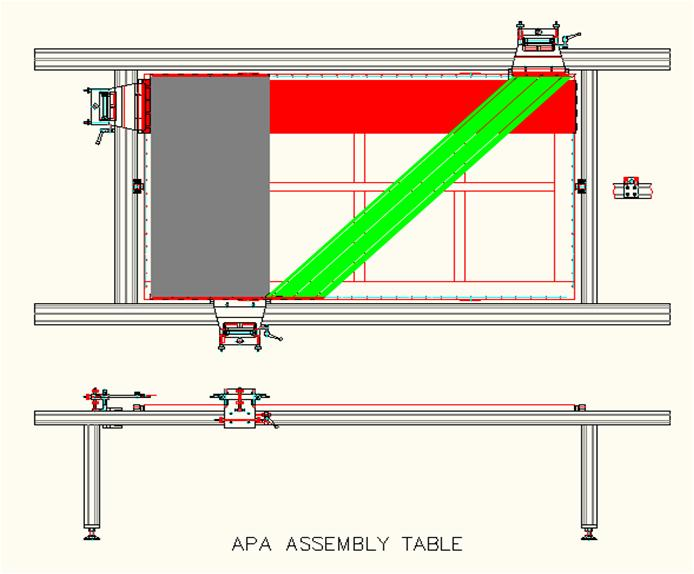
\includegraphics[width=\linewidth]{v5c3_APA_AD5}
\caption{Assembly table with equipment for stretching wires.}
\label{fig:tpc-APA-AD5}
\end{figure}
                          
Demonstration modules of both APA designs are being constructed. They will be evaluated to determine which design will be used in the final APA construction.

%%%%%%%%%%%%%%%%%%%%%%%%%%%%%%%%
\section{Cathode Plane Assemblies}
\label{subsec:v5-tpc-chamber-cathode}

The cathode plane assemblies (CPAs) have similar dimensions to the APAs, 
2.3~m wide and 6~m high. Each CPA is made of a stainless-steel framework, 
with a layer of stainless-steel wire mesh stretched over one side 
of the frame. To reduce drift-field distortion, all surfaces that rise
significantly above the mesh, including the stainless-steel 
frame structure on the other side of the mesh, are covered with 
field-shaping electrodes biased at appropriate voltages. 
Figure~\ref{fig:tpc-cathode-model} illustrates the concept of the 
CPA. 

\begin{editornote}
  Editor's Note: Figure~\ref{fig:tpc-cathode-model} shows the 2012 design. The design has evolved to a tubular member with stainless steel sheet.
\end{editornote}


\begin{figure}[htbp]
\centering
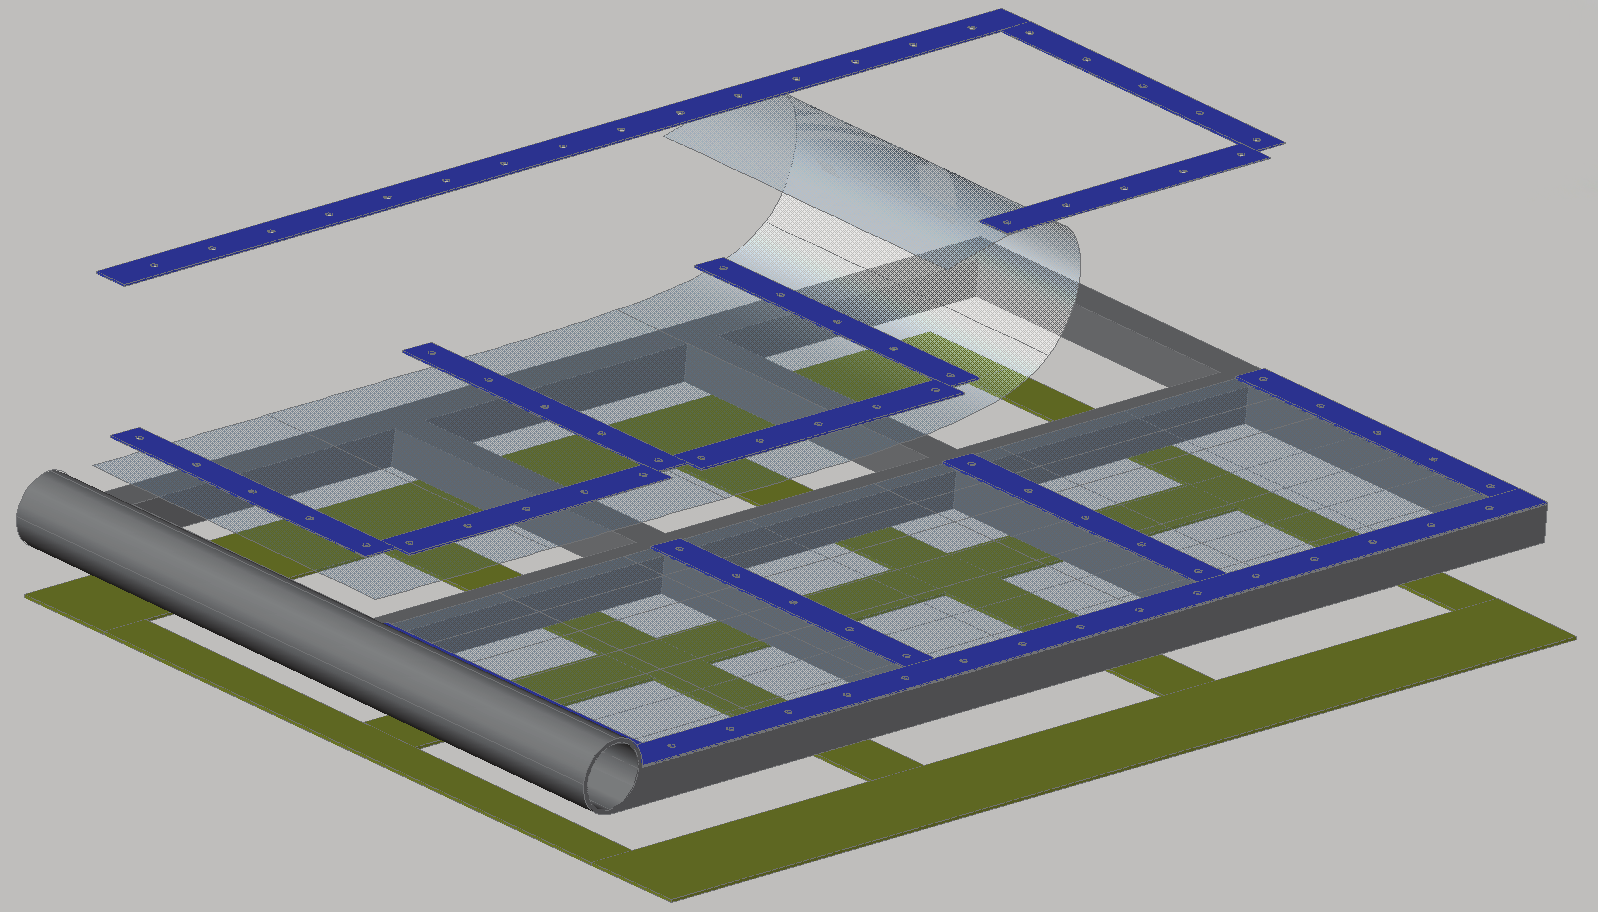
\includegraphics[width=\linewidth]{v5c3-tpc-cathode-model}
\caption[Conceptual design of a cathode plane assembly]{Conceptual design of a cathode plane assembly (not to scale). 
The assembly is 2.3~m wide and 6~m tall, similar to the APAs. As of December 2014 the design has evolved to a tubular member with stainless steel sheet. }
\label{fig:tpc-cathode-model}
\end{figure}

To achieve a 500~V/cm drift field over a 3.4~m distance, the bias 
voltage on the cathode plane must reach $-$170~kV. The minimal high-voltage 
bias system requires three high-voltage (HV) power supplies, one for each CPA 
row in the cryostat. Further partitioning of the CPA row and the field cages is being considered to reduce the loss of active volume in the event of HV failure inside the cryostat. For example, a six-zone configuration will require that a gap of several centimeters be maintained in the middle of each CPA row and field cage.  Failure to maintain HV in one zone will result in the loss of no more than 20\% of the active volume. 
%%%%%%%%%%%%%%%%%%%%%%%%%%%%%%%%
\section{Field Cage}
\label{subsec:v5-tpc-chamber-fieldcage}

Each pair of facing cathode and anode rows forms an electron-drift region. 
A field cage  completely surrounds the four open sides of this region
to provide the necessary boundary conditions to ensure a uniform electric field within, unaffected by the presence of the cryostat walls.

\begin{figure}[htbp]
\centering
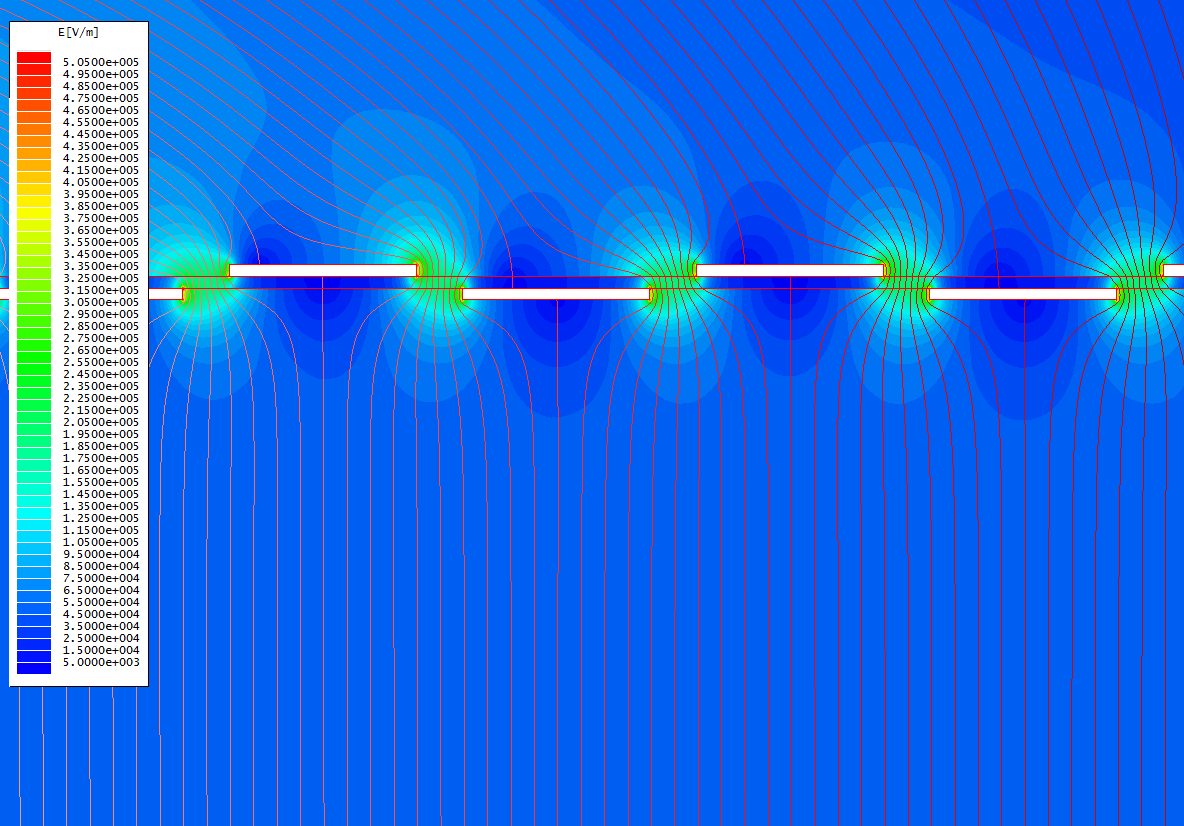
\includegraphics[width=4in]{v5c3-field-cage-simulation}
\caption[Electrostatic simulation of electric field near a section 
of field cage]{Electrostatic simulation of the electric field near a section 
of the field cage.  The filled color contours represent the electric 
field strength.  The line contours represent the electric
potential at 500~V intervals.  The pitch of the electrodes is 5~cm in this model. }
\label{fig:tpc-field-cage}
\end{figure}    

The entire TPC requires $\sim 1100 \rm{m}^2$ of field 
cage material per 5-kton detector. The field cages are constructed using copper-clad FR4 sheets reinforced with fiber glass I-beams to form panels of 2.5~m $\times$ 3.7~m in size. Parallel copper strips are etched/machined
on the FR4 sheets. Strips are 
biased at appropriate voltages provided by a resistive-divider network. These strips will create
a linear electric-potential gradient in the LAr, ensuring a uniform drift 
field in the TPC's active volume.  Figure~\ref{fig:tpc-field-cage} shows 
the results from an electrostatic simulation of a particular strip pattern. 
The drift-field non-uniformity quickly drops below 1\%, roughly 
a strip pitch away from the field-cage surface. Since the field cage 
completely encloses the TPC drift region on four (of six) sides, the FR4 sheets must 
be frequently perforated to allow natural convection of the liquid argon.  
The ``transparency'' of the perforation will be determined by a 
detailed LAr computerized fluid dynamic (CFD) study.

The resistor-divider network will be soldered directly onto the field-cage panels. 
Multiple resistors will be connected in parallel between any two taps of the divider,
in order to provide fault tolerance. 
One end of the divider chain is connected directly to the cathode, while the other end is connected to ground at the APA through resistors of the appropriate value. 

%%%%%%%%%%%%%%%%%%%%%%%%%%%%%%%%
\section{TPC Assembly in the Cryostat}

\begin{figure}[htbp]
\centering
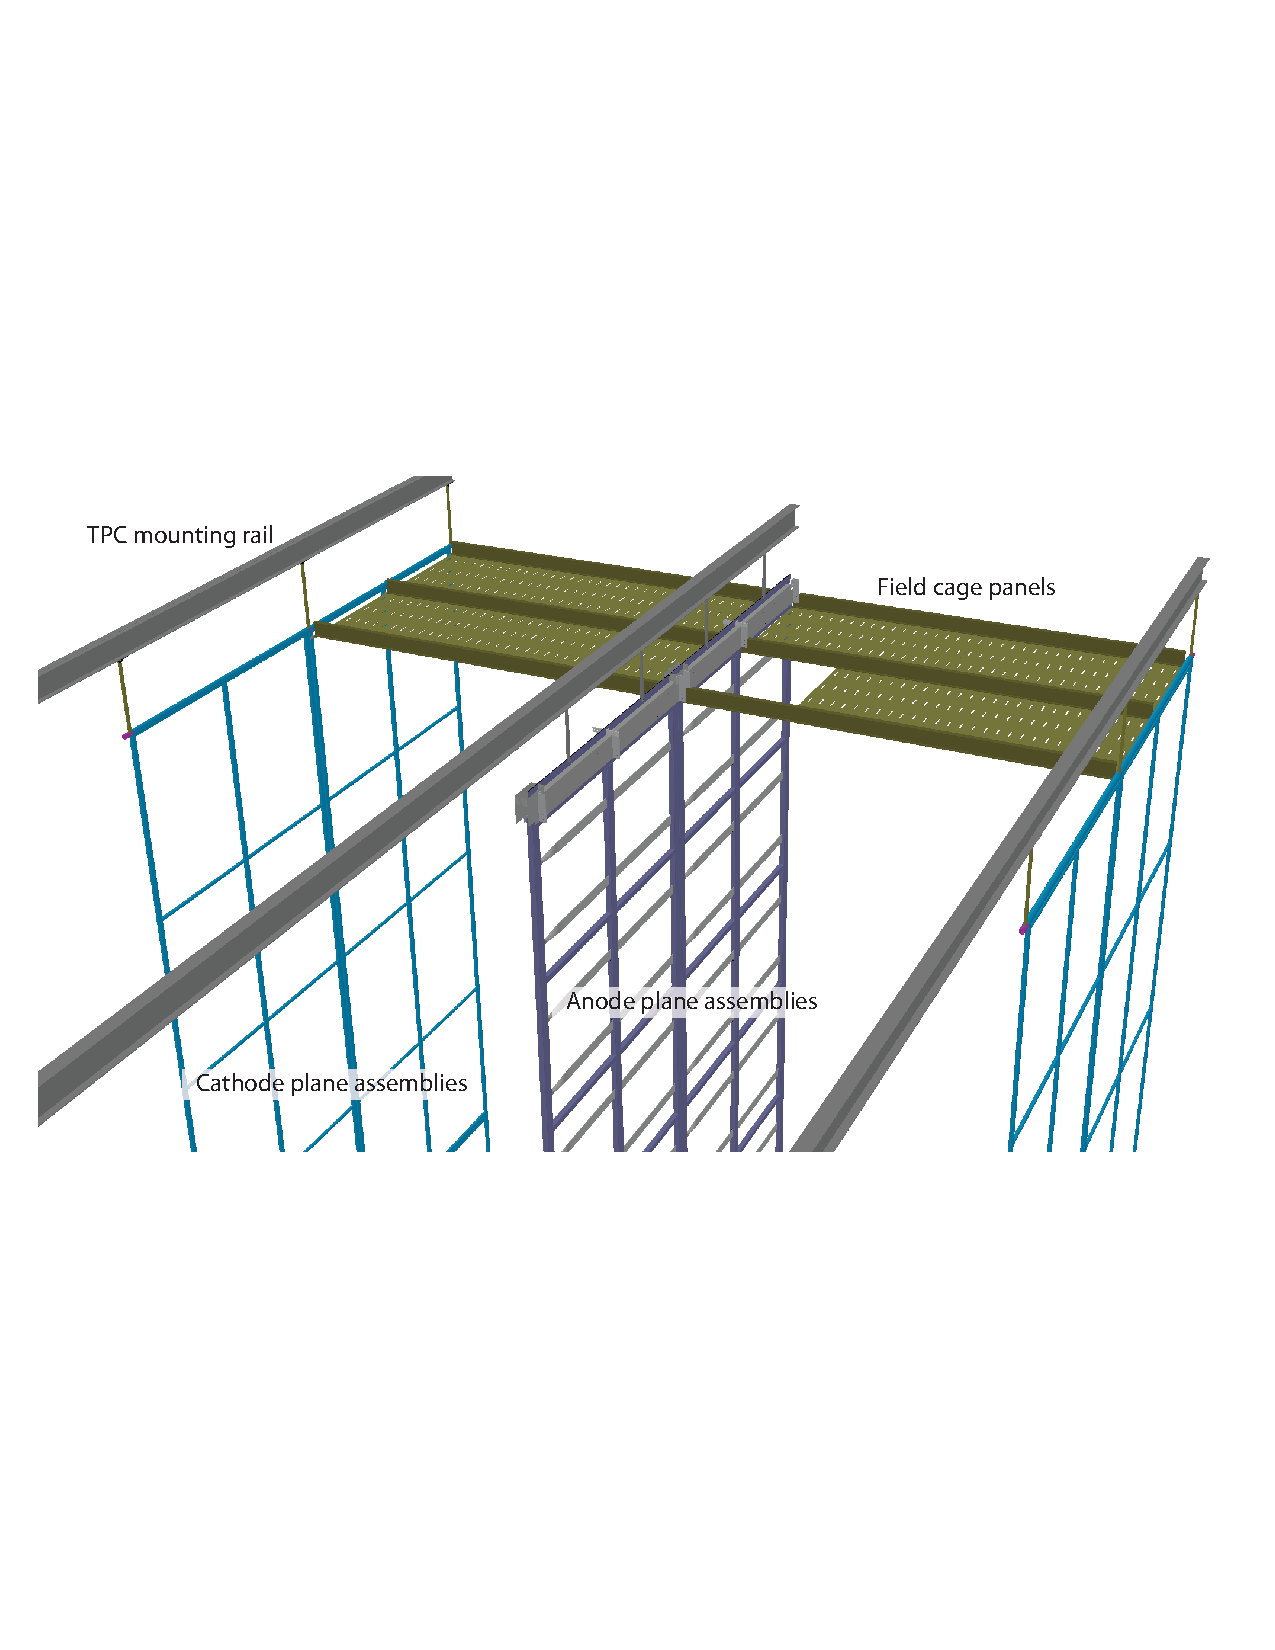
\includegraphics[width=\linewidth]{v5c3-tpc-partial-assembly}
\caption{A partial assembly of the TPC showing all major components}
\label{fig:tpc-partial-assembly}
\end{figure}

Figure~\ref{fig:tpc-partial-assembly} shows a partial assembly of a section of the TPC.
The finished cryostat has five rows of anchor points distributed along the ceiling (not shown in the figure). 
A mounting rail is suspended through stainless-steel rods to each row of the anchor points.  Under these five mounting rails, 
rows of CPAs and APAs are suspended in an interleaved fashion. 
Because the cathodes are at a high voltage, the CPAs are attached to their 
mounting rails through G10 rods. The distance between the facing anode and 
cathode is maintained by the pultruded fiberglass I-beams holding the FR4 sheets 
forming the field cage.  The TPC installation procedure 
is discussed in Chapter~\ref{ch:install}.

%%%%%%%%%%%%%%%%%%%%%%%%%%%%%%%%
\section{TPC Infrastructure}
\label{sec:v5-tpc-feedthru}

\begin{editornote}
  Editor's Note:  Some of the material in this section and the following subsections is now duplicated in the new CE chapter.
  This list below needs to be compared with the corresponding list in CE and revised.
\end{editornote}
   
The TPC infrastructure includes low-voltage and high-voltage supplies, all power cables and cable routing to the supplies, signal cables and cable routing to the DAQ, and all cryogenic feedthroughs.

%%%%%%%%%%%%%%%%
\subsection{Design Considerations} 
\label{subsec:v5-tpc-feedthru-reqs-n-specs}

\begin{itemize}
\item All power supplies must be able to be monitored and 
controlled both locally and remotely through the DAQ system.  
They must have over-current and over-voltage protection circuits.
\item The power supplies for the TPC cathode planes 
must be able to provide $-200$ kV at 1~mA current. The output voltage ripple 
must not introduce more than 10\% of the equivalent thermal noise from the front-end electronics. 
The power supplies must be programmable to trip (shutdown) 
their output at a certain current limit.  During power on and off, 
including output loss (for any reason), the voltage ramp rate at the 
feedthrough must be controllable to prevent 
damage to the in-vessel electronics through excess charge injection.
\item The power supplies for the wire-plane bias voltages
must provide sufficient current.   The output-voltage ripple 
must not introduce more than 10\% of the equivalent thermal noise from the front-end electronics. 
\item High-voltage feedthroughs must be able to withstand $-$250 kV 
at their center conductors in 1~atm air or argon gas environment when terminated in liquid argon.
\item Medium-voltage feedthroughs must be able to withstand twice their nominal operating voltages 
with a maximum specified leakage current in 1-atm argon gas.
\item Low-voltage power feedthroughs must be able to deliver 
sufficient DC current.
\end{itemize}

%%%%%%%%%%%%%%%%
\subsection{Reference Design} 
\label{subsec:v5-tpc-feedthru-desc}

There are three types of power supplies and matching 
feedthroughs in the cryostat: TPC high voltage, 
wire-bias voltages and low-voltage DC power to the readout electronics. There are two additional 
types of feedthroughs carrying digital signal: LVDS and optical fiber.

With the exception of the TPC high-voltage connections, all other 
cables inside the cryostat will be attached to their corresponding feedthroughs distributed throughout the cryostat roof.  The other ends of the cables will be connected to the matching connectors on the APAs in the cryostat.  The cables for the lower APAs must be carefully threaded through the hollow frames of the APA stacks.  The cables will be strain-relieved on the  mounting rails above the APAs. 

Measurements in the Materials Test Stand at Fermilab (described in Section~\ref{sec:mts})
have shown that impurities (principally O$_2$ and H$_2$O) embedded in objects submerged in the liquid argon do not result in a decrease in electron-drift lifetime, whereas impurities in objects located in the warmer gas phase do. This indicates the importance of minimizing the amount of material in the gas ullage at the top of the cryostat.  Therefore it may be desirable to connect all cables to feedthroughs below the liquid surface, and then pass the cables out of the cryostat, through an evacuated volume that traverses the gas and cryostat insulation, to a matching set of feedthroughs to the outside. 

%%%%%%%%%%%%%%%%
\subsection{TPC High Voltage }
\label{subsec:v5-tpc-feedthru-tpchv}

\begin{figure}[htbp]
\centering
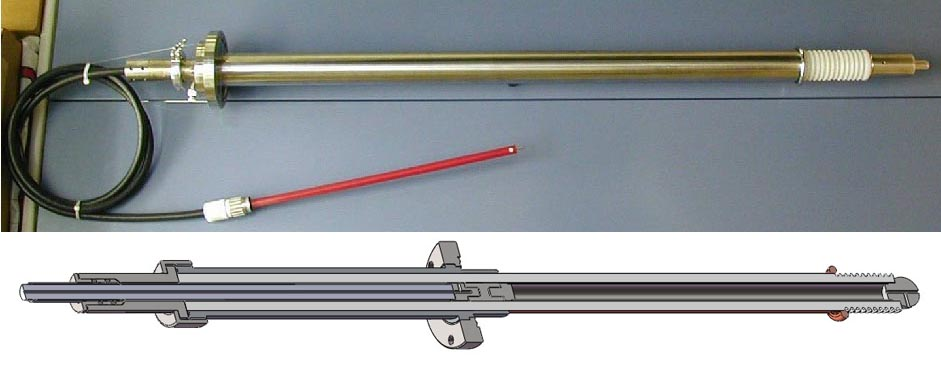
\includegraphics[width=\linewidth]{v5c3-feedthrough-hv.jpg}
\caption[ICARUS HV feedthrough; concept of new feedthrough]{Top: A high voltage feedthrough developed by the UCLA 
group for the Icarus experiment.  It was tested up to 150 kV.  Bottom: a conceptual design of a new feedthrough for the LAr-FD.}
\label{fig:tpc-UCLA-feedthrough}
\end{figure}

The cathode planes are biased at $-$170~kV to provide the required 
500~V/cm drift field. At a minimum, three high-voltage power 
supplies, each connecting through their own feedthroughs, will be used. Each supply will
provide high voltage to one of the three rows of the cathode plane assemblies.

The current candidate for the high-voltage power supplies is 
the Heinzinger PNC{\it hp} series, which is used by the ICARUS 
experiment.  Additional filtering of the voltage ripples is done through the intrinsic HV cable capacitance 
and series resistors. Established techniques and practices will be implemented to eliminate 
micro-discharges and minimize unwanted energy transfer in case of an HV breakdown. 
  
To ensure safe and reliable operation, the feedthroughs will be 
tested at a much higher voltage than expected in
routine operation ($\sim$ 250 kV) in liquid argon. 
 The feedthroughs will be 
mounted on the ceiling of the cryostat, their cold ends reaching 
through the gas ullage space and submerging into the liquid argon. 
The center conductor on the cold side of a feedthrough will be 
insulated and shielded by a grounded shroud at least 50~cm below the 
surface of the liquid. Connections between the feedthroughs 
and the CPA rows are made through stainless-steel pipes in the 
liquid argon. Figure~\ref{fig:tpc-UCLA-feedthrough} shows an example 
of a feedthrough made by the UCLA group for the ICARUS experiment, as well as the conceptual design of a feedthrough suitable for the LAr-FD TPCs.

\begin{figure}[htbp]
\centering
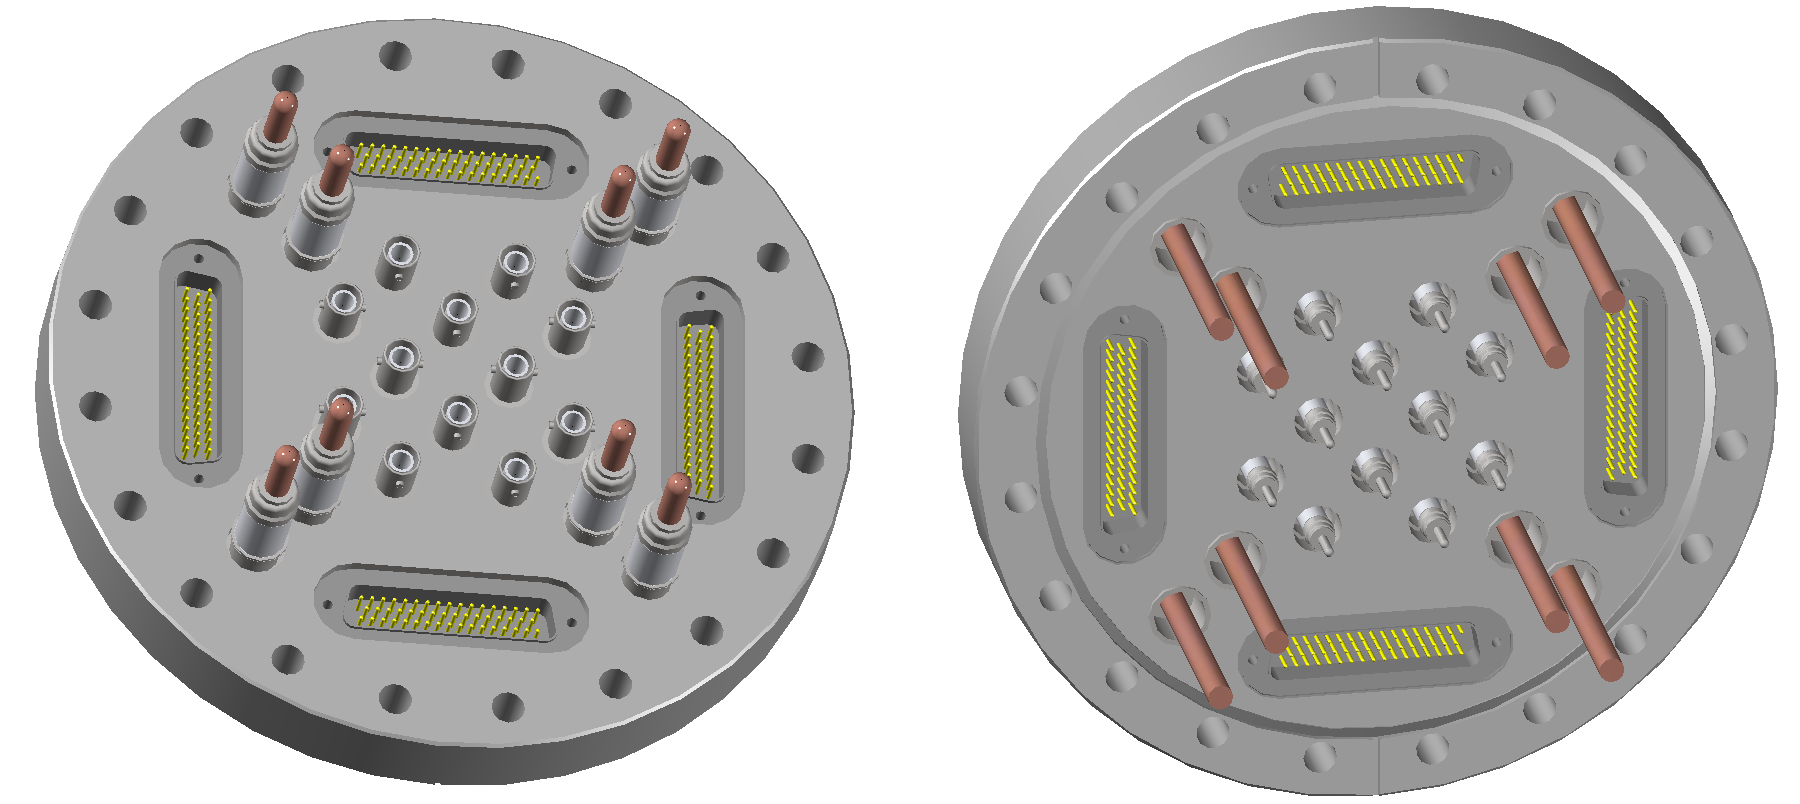
\includegraphics[width=\linewidth]{v5c3-signal-FT.png}
\caption[Conceptual design of signal/power feedthrough]{A conceptual design of a signal/power feedthrough using all off-the-shelf commercial components}
\label{fig:tpc-signal-feedthrough}
\end{figure}

%%%%%%%%%%%%%%%%
\subsection{Wire-Bias Voltages}
\label{subsec:v5-tpc-feedthru-wirebias}

Each anode plane assembly requires three bias voltage connections 
at $+$820V, $-$370V, and $-$665V.  The current on each of these 
supplies is expected to be zero at normal operation.  However the ripple 
voltage on the supply must be carefully controlled 
to avoid noise injection into the front-end electronics.  

The power supplies for the wire bias will be similar to 
those used for conventional multi-wire proportional chambers. 
Additional filtering networks will 
be needed to further reduce voltage ripples.  
The default feedthroughs are the commercial SHV type.  
However,  other, higher-density multi-channel 
feedthroughs capable of withstanding the maximum voltage are under investigation.  

%%%%%%%%%%%%%%%%
\subsection{Power for the Cold Electronics }
\label{subsec:v5-tpc-feedthru-power}

The power-per-channel for the front-end ASIC is designed to be about 15~mW and
the total power requirement for each APA is expected to be about 65~W.
Power will be supplied to the electronics on each APA separately by low-noise
power supplies outside the cryostat, either directly by
low-voltage (1.8~V), high-current (36 A) conductors or by high-voltage (48~V)
low-current (2~A) conductors to DC-DC converters placed locally in the LAr.
The use of DC-DC converters requires conductors with smaller cross section,
minimizing heat input to the cryostat (and ice formation of the feedthroughs).
However, the power dissipated by the (somewhat inefficient) converters in
the LAr will create boiling which may introduce contamination directly into the 
high-purity LAr, and if enough LAr is vaporized, may also produce strong mixing of the
ullage gas, driving more impurities into the liquid. These effects of boiling LAr, unless they can be demonstrated to be harmless, will drive a preference for eliminating DC-DC converters, and directly powering the front-end readout boards.

Heat conduction through the high-current feedthroughs and the self-heating ($I\cdot R$) of the wires are the factors contributing to additional heat load on the cryogenic system.   The sum of the these two factors as a function of the wire gauge, however, has a minimum 
due to the two opposing dependencies on the copper-wire cross section.  An optimum wire gauge can be chosen to minimize heat input to the cryostat.

%%%%%%%%%%%%%%%%
\subsection{Digital Data IO Feedthoughs}
\label{subsec:v5-tpc-feedthru-digital}

The TPC data rate per APA, using the zero-suppression and full event-buffer scheme described earlier, appears sufficiently low that it is within the capability of a single LVDS channel on copper. Optical fiber will be used if data must be transmitted at a much higher rate.  In this case, the number of optical fibers will be two per APA for redundancy, or 102 for each five-kton module. Commercial optical-fiber feedthroughs are available to meet this demand.

In addition to the high-speed data-output channels,  LVDS connections will be made to each APA to 
distribute a clock signal and control information.  These data 
can be transmitted at a lower bit rate, clearly within the
capabilities of LVDS. The number of channels for these signals 
are on the order of thousands in the entire detector, easily covered by commercial multichannel feedthroughs. 

A conceptual design of an APA signal/power feedthrough flange is shown in Figure~\ref{fig:tpc-signal-feedthrough}.  Based on a standard 8-in conflat flange with all commercial off-the-shelf components, each of these feedthroughs will serve the bias/power/digital IO needs of four APAs.  

%%%%%%%%%%%%%%%%%%%%%%%%%%%%%%%%
\section{TPC Prototyping, Test and  Checkout}
\label{sec:v5-tpc-checkout}

%%%%%%%%%%%%%%%%
\subsection{TPC Prototyping}
\label{sec:v5-tpc-checkout-prototype}

\begin{editornote}
  Editor's Note:  Some of the material in this section and the following subsections is now duplicated in the new CE chapter.
  This material needs to be compared with the corresponding material list in CE and revised.
\end{editornote}

Several prototype TPC modules will be constructed during the 
design phase.  The initial prototypes will be fraction scale or 
partial models of the APA and CPA.  The CPA prototype will be used 
to evaluate the wire-mesh tension and field-shaping electrode 
attachment techniques.   The APA prototype will be used to study 
the placement of the wire-wrapping boards and wire-support structures.  
It will also be used to develop the prototype winding machines.  
The prototypes will undergo numerous thermal cycles down to 
liquid-nitrogen temperature to test the integrity of the wire-to-board
and board-to-frame bonds.

The second set of prototypes will be scale models of the 
APA and CPA.  They will be used to validate the designs and 
to evaluate production procedures.  Prototype front-end electronics 
boards are expected to be available at this stage.  This TPC will be assembled in the 35-t prototype cryostat, expected to be operational in 2015.

A prototype that is proposed to go into the CERN neutrino beamline requires three full-size APAs with fully instrumented readout electronics, six full-size CPAs, and complete field-cage coverage.  The TPC will be constructed using identical APAs, CPAs and field-cage panels as designed for the LAr-FD.  Additional features will be installed to ensure proper TPC operation given the half-height cryostat configuration. The construction and assembly of all TPC mechanical components will use the same materials and techniques as designed for LAr-FD, with the exception of a reduced degree of automation that will be used to wire APAs for the LAr-FD.

A complete set of cold electronics will be installed on the APAs.  The electronics components will closely resemble those designed for the LAr-FD. All key features of the LAr-FD electronics chain, including preamp, shaper, ADC, digital buffer, zero suppression and multiplexing will be implemented.  Some  electronics  may be in prototype or functional-equivalent form.

%%%%%%%%%%%%%%%%
\subsection{Assembly Testing}
\label{sec:v5-tpc-checkout-test}

The front-end readout boards will be thoroughly tested.
\begin{itemize}
\item A small number of the ASICs will undergo a complete suite 
of tests, including thermal cycling to determine the batch yield.
\item If the yield is high ($>$ 95\%), all ASICs will be mounted 
on the front-end boards.  Tests will be performed on each board  
and bad chips replaced as needed.
\item If the yield is not high, an automated test fixture will be 
fabricated to validate every ASIC chip before mounting on the 
readout boards.  Board-level tests after mounting the
ASICs will be conducted.
\item The fully assembled front-end boards will be thermally cycled multiple times while connected to a simple DAQ system to ensure reliable operation.
\item The wire-carrier boards will be thermally cycled and HV stressed.
\end{itemize}

The APAs will also undergo testing.
\begin{itemize}
\item The tension and electrical continuity of each wire will be 
measured after the plane of wires is bonded to the frame.
\item After the front-end electronics boards have been installed on 
the APA, an initial calibration of all electronic channels will be 
performed.  The electronic gains and noise levels of all channels will be 
recorded in a database.
\item A cool-down stress test will be performed on each completed 
APA in a liquid-nitrogen environment.  Electronic calibration on 
all channels will be performed while the APA is cold and again
after it is warmed up.  Significant differences in the cold and warm calibration 
results will be investigated and remediated.  
\end{itemize}

For the CPAs, a cool-down stress test will be performed on each completed 
CPA in a LN2 environment.  After warming up, 
 the tension of the wire mesh will be checked.


For the field cages,  the resistance will be measured along each copper strip,  
and between strip pairs.  The resistance between two 
strips should exceed 1 G$\Omega$, without the resistive divider. 

%%%%%%%%%%%%%%%%
\subsection{Checkout } 
\label{sec:v5-tpc-checkout-checkout}

After passing the tests at the assembly level, the APAs will be 
put into storage, and later transported to the LBNE Far Site.  
Prior to installation, another round of electronic calibration will be 
performed on the APAs to validate their acceptable status.  

During installation, the DAQ system will be running continuously.  As soon 
as each stack of APAs is connected to the pre-routed cables, 
a suite of calibration runs will be performed to validate that all connections have
been made properly.  Repair or replacement at this stage will 
still be straightforward.

After the entire TPC is assembled, a system-wide calibration 
will be performed at room temperature and again at cryogenic 
temperature in argon gas.  Repair or replacement would
require partial disassembly of the TPC and should be avoided 
unless absolutely necessary.  

The responsibility and authority for the design, installation 
and use of the detector quiet-power distribution and 
detector-grounding system is held by the  
subproject electrical engineer. 
This engineer 
has oversight responsibility for all electrical and electronics 
design and installation tasks, including all attachments to the detector 
that create an electrical connection. 



